\documentclass[12pt]{report} \usepackage[T1]{fontenc} 
\usepackage[T1]{fontenc} % Better font encoding - must be early
\usepackage{lmodern} % Latin Modern fonts for better PDF resolution
\usepackage{geometry}
\geometry{a4paper, left=1in, right=1in, top=1in, bottom=1in}
\usepackage{graphicx}
\usepackage{setspace} % For setting line spacing
\usepackage{tabularx} % For flexible table width
\usepackage{array}
\usepackage{enumitem}
\usepackage{hyperref}
\usepackage{amssymb}
\usepackage{fancyhdr}
\usepackage{bookmark} % For setting destination for bookmarks
\usepackage{titlesec} % For customizing chapter titles
\usepackage{float}
\usepackage{fontawesome5} % For home icon
\usepackage{booktabs} % For professional table rules (\toprule, \midrule, \bottomrule)
\setcounter{secnumdepth}{3}  % Number up to subsubsection level
\setcounter{tocdepth}{3}     % Include subsubsections in TOC

% % Disable hyphenation
% \hyphenpenalty=10000
% \exhyphenpenalty=10000
% \tolerance=1
% \emergencystretch=\maxdimen
% \hbadness=10000

\pagestyle{fancy}
\fancyhf{}
\fancyhead[R]{\hyperlink{tableofcontents}{\faHome}} % Home icon to jump to Table of Contents
\fancyfoot[C]{\thepage} % Page number at the bottom center
\renewcommand{\headrulewidth}{0pt} % Remove header rule

\fancypagestyle{plain}{% Redefine the plain page style
    \fancyhf{} % Clear header/footer
    \fancyhead[R]{\hyperlink{tableofcontents}{\faHome}} % Home icon to jump to Table of Contents
    \fancyfoot[C]{\thepage} % Page number at the bottom center
    \renewcommand{\headrulewidth}{0pt} % Remove header rule
    \renewcommand{\footrulewidth}{0pt} % Remove footer rule
}

\hypersetup{
    colorlinks=true,
    linkcolor=blue,
    filecolor=magenta,      
    urlcolor=cyan,
    pdftitle={Edge AI Computing for Grape Leaf Disease Detection in LoRaWAN-Based Vineyard Monitoring System},
    pdfpagemode=FullScreen,
}

% Custom command to create hyperlinks
\newcommand{\customlink}[2]{\hyperlink{#1}{#2}}


\titleformat{\chapter}[display]
  {\normalfont\huge\bfseries\raggedright} % style for "Chapter 3"
  {Chapter \thechapter}
  {0pt}
  {\LARGE} % <-- chapter TITLE size
\titlespacing*{\chapter}{0pt}{*2}{*1}


  % 0pt left indent
  % 3.5ex before the section title
  % 2.3ex after the section title
\usepackage{titlesec}
% SECTION (Tighter)
\titleformat{\section}{\normalfont\large\bfseries}{\thesection}{1em}{}
\titlespacing*{\section}{0pt}{2.0ex plus 0.5ex minus .2ex}{0.2ex plus .2ex}
% SUBSECTION (Tighter)
\titleformat{\subsection}{\normalfont\normalsize\bfseries}{\thesubsection}{1em}{}
\titlespacing*{\subsection}{0pt}{1.5ex plus 0.5ex minus .2ex}{0.2ex plus .2ex}
% SUBSUBSECTION (Tighter)
\titleformat{\subsubsection}{\normalfont\normalsize\itshape}{\thesubsubsection}{1em}{}
\titlespacing*{\subsubsection}{0pt}{1.0ex plus 0.5ex minus .2ex}{0.1ex plus .2ex}


% Other package imports
\usepackage[english, italian]{babel}
\usepackage{geometry}
% Lingua per la bibliografia
\usepackage[fixlanguage]{babelbib}
% Codifica del testo
\usepackage[utf8]{inputenc} 
\usepackage{lipsum}
% Per ruotare le immagini
\usepackage{rotating}
% Per modificare l'header delle pagine 
\usepackage{fancyhdr} 
\usepackage[normalem]{ulem}

% Librerie matematiche
\usepackage{amssymb}
\usepackage{amsmath}
\usepackage{amsthm}
\usepackage[table,dvipsnames]{xcolor}         
\usepackage{listings}          
\usepackage{subcaption} 
\usepackage{threeparttable} 

% TikZ for flowcharts and diagrams
\usepackage{tikz}
\usetikzlibrary{positioning,arrows.meta,shadows,shapes.geometric}

% Define custom colors for TikZ diagrams
\definecolor{NavyBlue}{RGB}{0,51,102}
\definecolor{lightblue}{RGB}{220,235,250}

\singlespacing          % Single spacing (current default)
%\onehalfspacing         % 1.5 line spacing
%\doublespacing          % Double spacing
%\setstretch{1.25}       % Custom spacing 

% -----------------------------------------------------------------

% Modifica lo stile dell'header
\pagestyle{fancy}
\fancyhf{}
\lhead{\rightmark}
\rhead{\hyperlink{tableofcontents}{\faHome}}
\fancyfoot{}
\setlength{\headheight}{15pt}

% Rimuove il numero di pagina all'inizio dei capitoli
\fancypagestyle{plain}{
  \fancyfoot{}
  \fancyhead{}
  \renewcommand{\headrulewidth}{0pt}
}

% Stile del codice
\lstdefinestyle{codeStyle}{
    % Colore dei commenti
    commentstyle=\color{teal},
    % Colore delle keyword
    keywordstyle=\color{Magenta},
    % Stile dei numeri di riga
    numberstyle=\tiny\color{gray},
    % Colore delle stringhe
    stringstyle=\color{violet},
    % Dimensione e stile del testo
    basicstyle=\ttfamily\footnotesize,
    % newline solo ai whitespaces
    breakatwhitespace=false,     
    % newline si/no
    breaklines=true,                 
    % Posizione della caption, top/bottom 
    captionpos=b,                    
    % Mantiene gli spazi nel codice, utile per l'indentazione
    keepspaces=true,                 
    % Dove visualizzare i numeri di linea
    numbers=left,                    
    % Distanza tra i numeri di linea
    numbersep=5pt,                  
    % Mostra gli spazi bianchi o meno
    showspaces=false,                
    % Mostra gli spazi bianchi nelle stringhe
    showstringspaces=false,
    % Mostra i tab
    showtabs=false,
    % Dimensione dei tab
    tabsize=2
} \lstset{style=codeStyle}  
\lstdefinestyle{longBlock}{
    commentstyle=\color{teal},
    keywordstyle=\color{Magenta},
    numberstyle=\tiny\color{gray},
    stringstyle=\color{violet},
    basicstyle=\ttfamily\scriptsize,
    breakatwhitespace=false,         
    breaklines=true,                 
    captionpos=b,                    
    keepspaces=true,                 
    numbers=left,                    
    numbersep=5pt,                  
    showspaces=false,                
    showstringspaces=false,
    showtabs=false,                  
    tabsize=2
} \lstset{style=codeStyle}


\lstset{aboveskip=20pt,belowskip=20pt}
\hypersetup{
    colorlinks,
    linkcolor=CornflowerBlue,
    citecolor=CornflowerBlue
}

% Aggiunti definizioni, teoremi, linea e listing
\newtheorem{definition}{Definizione}[section]
\newtheorem{theorem}{Teorema}[section]
\providecommand*\definitionautorefname{Definizione}
\providecommand*\theoremautorefname{Teorema}
\providecommand*{\listingautorefname}{Listing}
\providecommand*\lstnumberautorefname{Linea}
\raggedbottom
% Include the 'titlesec' package
\usepackage{titlesec}

% Reduce vertical spacing before chapters
\titlespacing*{\chapter}{0pt}{-20pt}{40pt}
% Include the 'titlesec' package
\usepackage{titlesec}
% Reduce vertical spacing before and after chapters
\titlespacing*{\chapter}{0pt}{-20pt}{10pt}
\setlength{\parskip}{0.8em}
\setlength{\parindent}{0em}
\usepackage{titlesec}
% Include the 'fancyhdr' package for custom headers and footers
\usepackage{fancyhdr}
\fancypagestyle{plain}{% Apply to plain page style (used for chapter starts)
  \fancyhf{}
  \fancyhead[R]{\hyperlink{tableofcontents}{\faHome}}
  \fancyfoot[C]{\thepage}
}
\pagestyle{fancy}
\fancyhf{} % Clear all header and footer fields
\fancyhead[R]{\hyperlink{tableofcontents}{\faHome}} % Home icon to jump to Table of Contents
\fancyfoot[C]{\thepage} % Page number at the bottom center

% Set proper headheight to avoid warnings
\setlength{\headheight}{15pt}

%%%%%%%%%%%%%%%%%%%%%%%%%%%%%%%%%%%% Document begin %%%%%%%%%%%%%%%%%%%%%%%%%%%%%%%%%%%%%%%
\begin{document}

\begin{titlepage}
\begin{figure}[!htb]
    \centering
    
\includegraphics[keepaspectratio=true,scale=0.5]{images/cherubinFrontespizio.eps}
\end{figure}

\begin{center}
    \LARGE{UNIVERSITÀ DI PISA}
    \vspace{5mm}
    \\ \large{DIPARTIMENTO DI INGEGNERIA DELL’INFORMAZIONE}
    \vspace{2mm}
    \\ \LARGE{MASTERS IN ARTIFICIAL INTELLIGENCE AND DATA ENGINEERING}
\end{center}

\vspace{15mm}
\begin{center}
    {\large{ \textit{\textbf{ Edge AI Computing for Grape Leaf Disease Detection in LoRaWAN-Based Vineyard Monitoring System }}}}
    % Se il titolo è abbastanza corto da stare su una riga, si può usare
    
    % {\LARGE{\bf Un fantastico titolo per la mia tesi!}}
\end{center}
\vspace{30mm}

\begin{minipage}[t]{0.47\textwidth}
	{\large{Advisories:}\normalsize\vspace{3mm}
	\\ \large{Prof. Vallati Carlo} \normalsize\vspace{3mm}
    \\ \large{Dr. Palla Fabrizio} \normalsize\vspace{3mm}
    \\ \large{Prof. Zinnai Angela} \normalsize\vspace{3mm}}
\end{minipage}
\hfill
\begin{minipage}[t]{0.47\textwidth}\raggedleft
	{\large{Candidate:}\hspace{45mm}{\normalsize\vspace{3mm} \\ {Tsegay Teklay Gebrelibanos\\ID Number: 683925}}}
\end{minipage}

\vspace{5mm}
\hrulefill
\\\centering{\large{Academic Year 2025/2026}}

\end{titlepage}


\vfill % Fill the remaining vertical space
\usetikzlibrary{positioning, fit, calc, arrows.meta}
\newpage
\pagestyle{fancy}
% Header with home icon to navigate back to Table of Contents
\fancyhead[R]{\hyperlink{tableofcontents}{\faHome}}
\fancyfoot[C]{\thepage} % Page number at the bottom center

% Start main content with Roman numerals for front matter
\pagenumbering{roman}
\setcounter{page}{1}

% Explicitly set the language to English
\selectlanguage{english}

% ========================================
% FRONT MATTER
% ========================================

% Abstract
\phantomsection
\hypertarget{Abstract}{}
\chapter*{Abstract}
\addcontentsline{toc}{chapter}{Abstract}

% English Abstract
\section*{English}

Grapevine diseases pose a significant threat to global viticulture, causing substantial economic losses and compromising crop quality. Early and accurate disease detection is essential for effective disease management, yet traditional manual inspection methods are labor-intensive, subjective, and impractical for large-scale operations. While centralized cloud-based approaches using deep learning have demonstrated promising results, they require continuous network connectivity and introduce latency, making them unsuitable for remote vineyard environments.

This thesis presents the design and implementation of a fully autonomous edge AI system for real-time grape leaf disease detection deployed on resource-constrained ESP32-S3 microcontrollers. The system employs a two-stage deep learning pipeline: ESPDet-Pico, a YOLO-based lightweight object detection model, localizes individual grape leaves within captured images, followed by a fine-tuned MobileNetV2 classifier that identifies disease symptoms across four classes (Black Rot, Esca, Healthy, and Leaf Blight). To address the severe memory and computational constraints of embedded systems, both models undergo INT8 post-training quantization using the ESP-PPQ framework, reducing the detection model to 478 KB and the classification model to 2.73 MB while maintaining high accuracy.

A key innovation of this work is the hybrid weighted multi-leaf aggregation algorithm, which combines detection confidence, prediction entropy, and spatial quality metrics to synthesize robust disease predictions from multiple leaf observations within a single frame. This aggregation strategy achieves 98.7\% classification accuracy, representing a 3.4\% improvement over single-leaf predictions and reducing false positive rates by a factor of four.

The complete inference pipeline executes in 6.3 seconds per frame, including 78 ms for image capture, 366 ms for leaf detection, and 5.8 seconds for classifying up to ten detected leaves. Careful memory management enables operation within the ESP32-S3's 8 MB PSRAM, allocating buffers for camera DMA, JPEG frame storage, decoded RGB images, model activations, and processing intermediates. The system incorporates deep sleep power management with 5-minute duty cycles, achieving 20-25 days of autonomous operation on a 3000 mAh battery.

This research demonstrates the feasibility of deploying sophisticated deep learning models on ultra-low-cost microcontrollers for precision agriculture applications, offering a practical, scalable, and energy-efficient alternative to cloud-dependent solutions for vineyard disease monitoring.

\vspace{1cm}

\noindent\textbf{Keywords:} Edge AI, ESP32-S3, Deep Learning, Plant Disease Detection, YOLO, MobileNetV2, Model Quantization, Multi-Leaf Aggregation, Low-Power Computing, Precision Agriculture

\vspace{2cm}

% Italian Abstract
\section*{Riassunto}

Le malattie della vite rappresentano una minaccia significativa per la viticoltura globale, causando perdite economiche sostanziali e compromettendo la qualità delle colture. Il rilevamento precoce e accurato delle malattie è essenziale per una gestione efficace, tuttavia i metodi tradizionali di ispezione manuale sono laboriosi, soggettivi e impraticabili per operazioni su larga scala. Sebbene gli approcci centralizzati basati su cloud che utilizzano il deep learning abbiano mostrato risultati promettenti, richiedono connettività di rete continua e introducono latenza, rendendoli inadatti per ambienti viticoli remoti.

Questa tesi presenta la progettazione e l'implementazione di un sistema edge AI completamente autonomo per il rilevamento in tempo reale delle malattie delle foglie di vite, implementato su microcontrollori ESP32-S3 con risorse limitate. Il sistema utilizza una pipeline di deep learning a due stadi: ESPDet-Pico, un modello leggero di object detection basato su YOLO, localizza le singole foglie di vite all'interno delle immagini acquisite, seguito da un classificatore MobileNetV2 ottimizzato che identifica i sintomi delle malattie in quattro classi (Black Rot, Esca, Sana e Leaf Blight). Per affrontare i severi vincoli di memoria e calcolo dei sistemi embedded, entrambi i modelli subiscono una quantizzazione INT8 post-training utilizzando il framework ESP-PPQ, riducendo il modello di detection a 478 KB e il modello di classificazione a 2,73 MB mantenendo un'elevata accuratezza.

Un'innovazione chiave di questo lavoro è l'algoritmo di aggregazione multi-foglia con pesi ibridi, che combina la confidenza di detection, l'entropia della predizione e le metriche di qualità spaziale per sintetizzare previsioni robuste dalle osservazioni di più foglie in un singolo frame. Questa strategia di aggregazione raggiunge un'accuratezza di classificazione del 98,7\%, rappresentando un miglioramento del 3,4\% rispetto alle predizioni su singola foglia e riducendo i tassi di falsi positivi di un fattore quattro.

La pipeline di inferenza completa viene eseguita in 6,3 secondi per frame, includendo 78 ms per l'acquisizione dell'immagine, 366 ms per il rilevamento delle foglie e 5,8 secondi per la classificazione di fino a dieci foglie rilevate. Una gestione accurata della memoria consente l'operazione all'interno degli 8 MB di PSRAM dell'ESP32-S3, allocando buffer per il DMA della camera, la memorizzazione dei frame JPEG, le immagini RGB decodificate, le attivazioni del modello e gli intermedi di elaborazione. Il sistema incorpora una gestione energetica con deep sleep e cicli di lavoro di 5 minuti, raggiungendo 20-25 giorni di funzionamento autonomo con una batteria da 3000 mAh.

Questa ricerca dimostra la fattibilità di implementare modelli sofisticati di deep learning su microcontrollori a bassissimo costo per applicazioni di agricoltura di precisione, offrendo un'alternativa pratica, scalabile ed efficiente dal punto di vista energetico alle soluzioni dipendenti dal cloud per il monitoraggio delle malattie nei vigneti.

\vspace{1cm}

\noindent\textbf{Parole chiave:} Edge AI, ESP32-S3, Deep Learning, Rilevamento Malattie delle Piante, YOLO, MobileNetV2, Quantizzazione del Modello, Aggregazione Multi-Foglia, Computazione a Basso Consumo, Agricoltura di Precisione

\newpage

% Acknowledgments
\chapter*{Acknowledgments}
\addcontentsline{toc}{chapter}{Acknowledgments}

% TODO: Personalize your acknowledgments

I would like to express my sincere gratitude to my supervisor, Prof. [Supervisor Name], for their invaluable guidance, continuous support, and insightful feedback throughout this research work.

I am deeply grateful to the team at INFN (Istituto Nazionale di Fisica Nucleare) for providing me with the opportunity to work on this challenging and rewarding project. Special thanks to [Co-supervisor/Mentor Name] for their technical expertise and mentorship during the development and implementation phases.

I would like to thank my family for their unwavering support and encouragement throughout my academic journey.

Finally, I acknowledge the use of computational resources and datasets that made this work possible.

\vspace{1cm}

\begin{flushright}
Tsegay\\
University of Pisa\\
February 2026
\end{flushright}

\newpage

% Label for Table of Contents
\phantomsection
\hypertarget{tableofcontents}{}
\tableofcontents
\newpage

% List of Figures
\phantomsection
\addcontentsline{toc}{chapter}{List of Figures}
\listoffigures
\newpage

% List of Tables
\phantomsection
\addcontentsline{toc}{chapter}{List of Tables}
\listoftables
\newpage

% List of Acronyms
\chapter*{List of Acronyms}
\addcontentsline{toc}{chapter}{List of Acronyms}

\begin{table}[H]
\centering
\begin{tabular}{ll}
\hline
\textbf{Acronym} & \textbf{Definition} \\ \hline
AI & Artificial Intelligence \\
CNN & Convolutional Neural Network \\
DL & Deep Learning \\
DMA & Direct Memory Access \\
ESP & Espressif Systems Processor \\
FP & False Positive \\
FP32 & 32-bit Floating Point \\
GPU & Graphics Processing Unit \\
INT8 & 8-bit Integer Quantization \\
IoT & Internet of Things \\
LoRaWAN & Long Range Wide Area Network \\
LPWAN & Low Power Wide Area Network \\
mAP & mean Average Precision \\
MCU & Microcontroller Unit \\
ML & Machine Learning \\
NN & Neural Network \\
ONNX & Open Neural Network Exchange \\
OTA & Over-The-Air \\
PTQ & Post-Training Quantization \\
PSRAM & Pseudo-Static Random Access Memory \\
RAM & Random Access Memory \\
ROI & Region of Interest \\
SRAM & Static Random Access Memory \\
TFLite & TensorFlow Lite \\
UART & Universal Asynchronous Receiver-Transmitter \\
WSN & Wireless Sensor Network \\
YOLO & You Only Look Once \\ \hline
\end{tabular}
\end{table}

\newpage

% Switch to Arabic page numbering for main content
\pagenumbering{arabic}

% ========================================
% MAIN BODY
% ========================================

% Label for chapters
\hypertarget{Chapter_1}{}
\chapter{Introduction and Background}
\label{chap:introduction}
Cultivation of grapes is one of the most economically significant crops in the world, as they are used for producing wine, juice, and also fresh fruit markets~\cite{mathew2025real}. However, as cultivation expands globally, disease issues increasingly threaten yield and quality, destabilizing the industry ~\cite{liu2025grape, mathew2025real}. Grape faces challenges from fungal and bacterial diseases including  Black Rot, Esca, Leaf Blight, and others can affect the entire harvest if not detected and managed promptly ~\cite{mathew2025real, talaat2025deepleaf, zhou2025lightweight, atesoglu2025detection}. The traditional disease identification relies on manual inspection by experts, which is laborious and vulnerable to error through human oversight~\cite{dharrao2025efficient}. In response to these limitations, The transition toward precision agriculture which is characterized by data driven management practices that has emerged as a critical paradigm shift to address these challenges~\cite{hnatiuc2023intelligent, aher2025deep}. Within this context, the development of intelligent monitoring systems capable of providing real time insights into plant health status has become increasingly vital for sustainable vineyard management.

The existing vineyard monitoring system is developed as a long-range, low-power wireless sensor network (WSN) platform for environmental monitoring and management of vineyards, aiming to provide methods to evaluate and improve the energy consumption of sensor nodes. The goal of this monitoring system is to provide an efficient and reliable way to promptly detect conditions adverse to grapes by measuring environmental data such as temperature, pressure, soil moisture, and humidity levels of vineyard fields. The platform is composed of a set of data acquisition sensors scattered over large open field areas, a gateway node, and a remote server to process and store the acquired data as shown in Figure~\ref{fig:lora}. This monitoring platform is based on the LoRaWAN specification, which is suitable for long-range and low-power lossy networks (LLNs) applications and provides a reliable link layer protocol for the deployed end nodes (sensor nodes) to access and transmit data to a central gateway, forming a star network topology~\cite{almufareh2024intelligent, jose2025lorawan}. The gateway node provides IP connectivity, forwarding the frames from the wireless sensor network to a local application server, which then sends the data to the LoRaWAN network server called The Things Stack. The telemetry data at the servers is gathered, stored in a MongoDB database, and displayed on a Grafana dashboard back to users, providing flexibility in the use and access of measured environmental conditions.

\begin{figure}[htbp]
   
    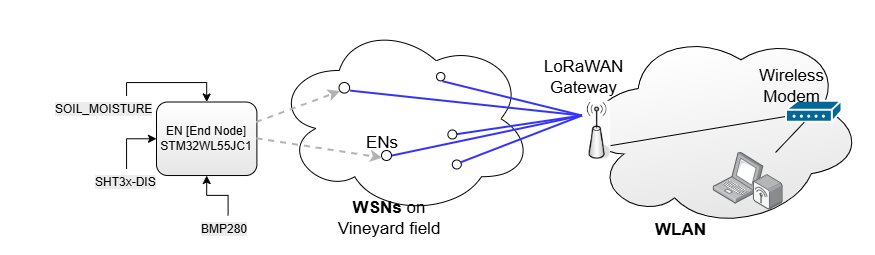
\includegraphics[width=0.7\linewidth]{images/lora2.drawio.png}
    \caption{\ LoRaWAN-based vineyard monitoring system architecture that only relies on environmental data for disease risk assessment}
    \label{fig:lora}
\end{figure}

Although the existing LoRaWAN-based vineyard monitoring system has showed significant potential for long term data collection across large field areas using low power communication, a fundamental limitation is still existing in this current implementations~\cite{gawande2024early, hnatiuc2023intelligent}. As some studies noted, a system with primarily rely on environmental data collection such as temperature, humidity, and pressure, transmitted over LoRaWAN networks and providing limited insights into the actual grapevine's health status~\cite{hnatiuc2025aiot}. Environmental sensing alone provides only indicators of disease risk rather than direct assessment of plant health. This gap of LoRaWAN-based vineyard monitoring system, not visualizing the actual grape leaf status, is representing there is a critical barrier to achieving more intelligent and responsive vineyard management systems.  


Meanwhile, deep learning models for identifying plant diseases have showed remarkable performance in laboratory and controlled environments. This is based on a comprehensive review of deep learning for grape leaf disease detection~\cite{aher2025deep}. This review shows convolutional neural networks and transformer based architectures can achieve high accuracy on detecting grape leaf diseases~\cite{karthik2024grapeleafnet, talaat2025deepleaf}. The Object detection frameworks such as YOLO also went further enabling automated leaf localization and disease symptoms in a complex field scenes~\cite{yang2024detection, chen2024yolov8}. Despite these advancements, the practice of deploying these models in vineyard monitoring systems remains limited due two critical challenges. First, The nature of  deep learning models typically demands high computational resources such as memory, processor and power, which is beyond the capabilities of the edge microcontroller~\cite{junaidi2025deep}. Second, the LoRaWAN network also have payload size constrains, transmitting raw image data is not feasible. 

Edge computing and lightweight deep learning (TinyML) becomes as a promising solution to address the computational resource and bandwidth limitations in LoRaWAN-based agricultural IoT systems. By performing image processing and inference at the sensor level. As prior studies explored, the lightweight vision models for disease detection in such resource-limited settings requires careful balance between model capacity and computational constraints~\cite{joshi2024edge, santhosh2024edge, junaidi2025deep}. However, most  of the  edge-based plant disease detection systems have been implemented on single-board computers such as Raspberry Pi or NVIDIA Jetson or smartphones, which offers mush more computational resources than microcontrollers~\cite{karim2024enhancing, lazcano2025deep, tao2025icrop+, mamun2025grape}.
 Therefore, such kinds of edge computing are not suitable for vineyard monitoring system which requires the edge computing for long term and battery powered deployment. 


To address this gap and to further enhance the intelligence of the existing vineyard monitoring system, this research came up with extension feature focused on edge computing for grape leaf disease detection. This extension Integrated edge AI at sensor level, moving beyond the traditional environmental monitoring, for nearly real-time visual-based insights into grapevines. By processing leaf images and running CNN classification model at the edge sensor, the system improves its ability to identify grape diseases. This differentiates the monitoring system from other systems that only rely on environmental data, thereby providing a more intelligent and efficient solution for vineyard management. This visual-based disease detection necessitates the tactical use of Edge AI computing to overcome the bandwidth limitations inherent in LoRaWAN communication for transmitting image data. Using ESP32-S3’s Edge AI capabilities, which support AI and can process images, the development process applied optimized configuration and enabled real-time grape leaf detection and classification directly at the edge sensor. This approach reduced power consumption by transmitting only the output of the MobileNet classification model, e.g. “Leaf Blight” with confidence 90\%, which is then seamlessly appended to the existing LoRaWAN data frame. Besides, by setting specified periodic intervals for image capture and on-device processing, followed by extended sleep periods (duty cycle operation) for the edge node, it aligns perfectly with a low-power, event-driven monitoring strategy, providing actionable insights while minimizing the impact on battery lifetime. Moreover, this comprehensive approach enhances the vineyard monitoring system by enabling early, localized detection of plant health issues, supporting more responsive and targeted interventions in precision agriculture.


Therefore, main aim of this research was to design, implement, and validate Edge AI system for grape leaf disease detection deployed on microcontroller within the existing LoRaWAN-based vineyard monitoring system. Specifically, this research introduces the direct visual-based disease detection into the existing environmental only monitoring system, by deploying a complete inference pipeline on ESP32-S3 microcontroller. Then the system integrates image acquisition, leaf localization within complex vineyard scenes, Multi-class disease classification, and inference results formatted to fit within LoRaWAN payload. Hence, contribution of this study have been diverse, addressing both technical and practical challenges of edge AI deployment for precision agriculture. It demonstrated feasibility of deploying these two-stage, object detection then classification pipeline on ESP32 microcontroller under strict  computing resources constraints.  This is a significant advancement beyond existing implementations that rely on powerful single-board computers or smartphone devices~\cite{karim2024enhancing, lazcano2025deep, mamun2025grape}.. Also introduces a weighted aggregation on the classification results from multiple leaves within a single frame, to send a compacted and robust results over LoRaWAN communication. overall, this work provide a complete system achitecture that fills the gap between enviromental only monitoring and direct disease detection. this research establised a foundation for Intelligent precision agricultural systems that combine the reliability of LoRaWAN with the optimized deep learning models deployed at the edge.

The Thesis organized in five chapters. Chapter 1 introduction and background of the research, outlining the research gap, main aim, and contributions of the study. Chapter 2 reviews some related works in the fields of IoT, LoRaWAN for precision agriculture, deep learning and edge computing for plants disease detection. Chapter 3 detailed system design implementation, including hardware selection, model architecture, dataset preparation, traning process, and integration with the existing LoRaWAN-based monitoring platform. Chapter 4 presents the experimental setup, evaluation metrics, and results of the system validation in both controlled and field conditions. Finally, Chapter 5 concludes the thesis by summarizing the findings, discussing implications for precision agriculture, and outlining directions for future research.

% The existing vineyard monitoring is developed in a long-range, low-power, wireless sensor network (WSN) platform for environmental monitoring and management of vineyards, aiming to provide methods to evaluate and improve the energy consumption of the sensor nodes. The goal of this monitoring system is to provide an efficient and reliable way to detect conditions adverse to the grapes by measuring environmental data such as temperature, pressure, soil mixture, and humidity levels of the vineyard fields. The platform is composed of a set of data acquisition sensors scattered over large open-field areas, a gateway node, and a remote server to process and store the acquired data. This monitoring platform is based on the LoRaWAN specification, which is suitable for long-range and low-power and lossy networks (LLNs) applications and provides a reliable link layer protocol for the deployed End Nodes (sensor nodes) to access and transmit data to a central gateway, forming a star network topology. The gateway node provides IP connectivity, forwarding the frames from the wireless sensor network (WSN) to a local application server, which then sends the data to the LoRaWAN Network server called The Things Stack Running from INFN's VM. The telemetry data at the servers is, gathered, stored in the MongoDB database, and displayed on the Grafana dashboard  back to the Users, providing flexibility in the use and access of the measured environmental conditions.

% Extension: Integrating Edge AI Computing for Grape Leaf Disease Detection
% To further enhance this vineyard monitoring system’s intelligence, this research adds an extension feature focused on edge computing for grape leaf disease detection. This feature Integrated edge AI at the sensor level, moving beyond the traditional environmental monitoring, for nearly real-time visual-based insights into grape leaves. By processing leaf images and running CNN classification model at the edge sensor, the system improves its ability to identify grape diseases. This differentiates the monitoring system from other systems that only rely on environmental data, thereby providing a more intelligent and efficient solution for vineyard management.

% The visual-based disease detection necessitates the tactical use of Edge AI computing to overcome the bandwidth limitations inherent in LoRaWAN communication for transmitting image data. Even though LoRaWAN excels at transmitting concise data frames for environmental readings, raw image transmission is too power-hungry and impractical for a low-power WSN. Utilizing the ESP32-S3’s Edge AI capabilities, which support AI and can process images, the development process becomes more flexible and efficient, enabling real-time grape leaf detection and classification directly at the edge sensor. This approach reduces power consumption by transmitting only the output of the clas- sification CNN, e.g. “Leaf Blight” with confidence 90\%, which is then seamlessly appended to the existing LoRaWAN data frame. Besides, by setting specified periodic intervals for image capture and on-device processing, followed by extended sleep periods (duty cycle operation) for the edge node, it aligns perfectly with a low-power, event-driven monitoring strategy, providing actionable insights while minimizing the impact on battery lifetime. Moreover, this comprehensive approach enhances the vineyard monitoring system by enabling early, localized detection of plant health issues, supporting more responsive and targeted interventions in precision agriculture.













\hypertarget{Chapter_2}{}
\chapter{Literature Review}
\section{Literature Review}
\subsection{Grape leaf disease detection using deep learning techniques}











\hypertarget{Chapter_3}{}
\chapter{{Edge AI System Design \& Implementation}}

\section{System Overview and Methodology}

This chapter presents the design, implementation, and deployment of an edge AI-based grape leaf disease detection system into existing vineyard monitoring infrastructure. The proposed system extends conventional LoRaWAN-based wireless sensor networks, which monitors only environmental parameters, by integrating sensor-level deep learning inference to enable real-time plant health status assessment.



\subsection{Four-Stage Pipeline Architecture}

The disease detection system is implemented in a four-stage pipeline deployed on ESP32-S3 microcontrollers, as illustrated in Figure~\ref{fig:system_architecture}.

\begin{figure}[htbp]
    \centering
    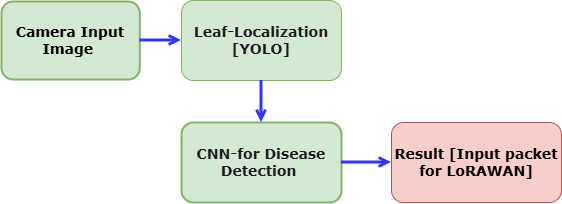
\includegraphics[width=0.75\linewidth]{images/system_architecture.png}

    \caption{Four-stage edge AI pipeline for grape leaf disease detection.}
    \label{fig:system_architecture}
\end{figure}

\textbf{Stage 1: Image Acquisition} -- An OV3660 camera module captures vineyard images at VGA resolution. The camera's built-in hardware JPEG encoder compresses images on-chip before transfer to the ESP32-S3.

\textbf{Stage 2: Leaf Localization} -- A YOLO-based detection model (ESPDet-Pico) localizes individual grape leaves within the captured frame. This stage identifies and crops leaf regions of interest, filtering out background elements. The ESP-optimized model architecture and training procedure are detailed in Section~\ref{sec:espdet_pico}.

\textbf{Stage 3: Disease Classification} -- Each detected leaf is resized and classified by a MobileNetV2 model fine-tuned on grape disease images. The two-stage transfer learning strategy and model evaluation are presented in Section~\ref{sec:mobilenetv2}.

\textbf{Stage 4: Multi-Leaf Aggregation} -- Since frames contain multiple leaves, predictions are aggregated using weighted combination of detection confidence, classification entropy, and spatial quality metrics. The aggregated result is encoded into a 16-byte LoRaWAN packet. The aggregation strategy and its effectiveness are analyzed in Chapter~\ref{chap:results}.



\section{Dataset Acquisition and Preparation}
\label{sec:dataset}
\vspace{-1mm}
In training the two distinct models, two separate datasets were used. The dataset for disease classification contains only single leaf images in a clear background, while the dataset for leaf localization contains images of natural vineyard scenes with annotated leaf bounding boxes. The reason for having two separate datasets is that the disease classification model is trained on a controlled dataset to learn disease-specific features on single leaf without background noise. But in practice the input image is natural vineyard scene with multiple leaves and complex background, so the leaf localization model is trained on a different dataset that reflects the deployment conditions to learn to localize leaves in unconstrained environments. Then the disease classification model is applied only on the detected \& cropped leaf regions obtained from the localization model, which is why it is trained on single leaf images. This separation allows each model to specialize in its respective task while ensuring that the overall system can handle real-world vineyard imagery effectively.
\vspace{-2mm}
\subsection{The Grape-Leaf Disease Dataset}
\vspace{-2mm}
The grape-leaf disease dataset obtained from the PlantVillage Dataset hosted on Kaggle~\cite{plantvillage_dataset_2023}, created by Abdallah Ali. PlantVillage is a widely-adopted public repository of plant disease imagery developed through collaborative citizen science efforts. The grape leaf subset aggregates pathology images captured under controlled laboratory conditions, ensuring consistent lighting and background characteristics. The dataset emphasizes leaf-level disease manifestations across four epidemiologically significant categories affecting viticulture worldwide. The dataset contains 4,062 RGB images and is distributed across four distinct disease classes: \textit{Black Rot} (caused by \textit{Guignardia bidwellii}), \textit{Esca} (Black Measles, a complex disease involving multiple fungal pathogens), \textit{Leaf Blight} (Isariopsis Leaf Spot, caused by \textit{Pseudocercospora vitis}), and  finally the \textit{Healthy class} (disease-free sample of grape leaves). Table~\ref{tab:classification_dataset_distribution} presents the complete class distribution statistics. 

\begin{table}[htbp]
\centering
\caption{Grape leaf disease dataset distribution across training, validation, test splits}
\label{tab:classification_dataset_distribution}
\begin{tabular}{lrrrr}
\toprule
\textbf{Disease Class} & \textbf{Training} & \textbf{Validation} & \textbf{Test} & \textbf{Total} \\
\midrule
Black Rot              & 803               & 141                 & 236           & 1,180          \\
Esca (Black Measles)   & 940               & 166                 & 277           & 1,383          \\
Healthy                & 287               & 51                  & 85            & 423            \\
Leaf Blight            & 731               & 129                 & 216           & 1,076          \\
\midrule
\textbf{Total}         & \textbf{2,761}    & \textbf{487}        & \textbf{814}  & \textbf{4,062} \\
\bottomrule
\end{tabular}
\end{table}

The dataset employs a fixed 80/20 train-test split at the top level, allocating 3,248 images for model development and 814 images for final evaluation. Stratified sampling ensures proportional class representation in both partitions, maintaining the original class distribution ratios. The development partition (3,248 images) is further subdivided into 85\% for training (2,761 images) and 15\% for validation (487 images), as detailed in Table~\ref{tab:classification_dataset_distribution}. This three-way split enables hyperparameter tuning on the validation set while preserving the test set for unbiased performance evaluation. All splits maintain class balance through stratified partitioning to prevent training bias toward majority classes.

\subsection{Grapevine Dataset for Leaf Localization}

The leaf localization dataset is used to train a model to identify grape leaf regions of interest (ROI) within unconstrained vineyard imagery. Unlike the classification dataset's controlled backgrounds, this dataset includes natural vineyard scenes with complex backgrounds, occlusions, and varying lighting conditions. These base images are sourced from the Grape/Grapes dataset on Kaggle~\cite{kaggle_grape_images_2023}, curated by Nicolaas Regnier. This collection contains 531 natural vineyard photographs capturing real-world deployment conditions with varying leaf densities, overlaps, lighting conditions, and background complexity. Unlike the disease classification dataset, which contains single leaves on uniform backgrounds, this collection captures the unstructured complexity of real vineyard environments, essential for training robust leaf localization models.

To adapt this dataset for object detection training, the images were manually annotated with bounding boxes of individual grape leaf regions. The annotation process was conducted using the Roboflow platform and segment anything model (SAM), where each leaf instance within the images was labeled with precise bounding box coordinates. These annotations are based on the YOLO format, each bounding boxes are specified by normalized center coordinates $(x_c, y_c)$, width $w$, and height $h$, all scaled to $[0, 1]$ relative to image dimensions. This normalization ensures resolution-independent annotation representation, facilitating training across variable input sizes. The annotated dataset, titled ``Grape Leaf ROI Detection'' is publicly published on Roboflow platform~\cite{roboflow_grape_leaf_2026}. The dataset exported in YOLOv11 format compatible with modern object detection frameworks. This dataset partitioned into training (328 images), validation (82 images), and test (103 images) sets, maintaining the natural distribution of leaf counts and scene complexity across splits. 


\subsection{Preprocessing and Augmentation Pipeline}

Data preprocessing and augmentation strategies differ substantially between the classification and detection tasks due to their distinct architectural requirements, input constraints, and training objectives.

\subsubsection{Input Resolution and Preprocessing}

Hardware memory limitations of the ESP32-S3 platform impose strict constraints on input resolution selection. The classification model operates on $128 \times 128$ pixel inputs, balancing model expressiveness with PSRAM availability for activation storage during inference. The detection model processes rectangular inputs at $416 \times 320$ pixels (aspect ratio 1.3:1), selected to accommodate the OV3660 camera's VGA output while maintaining computational efficiency for multi-object detection.

For classification, training images undergo \texttt{RandomResizedCrop} to $128 \times 128$ pixels, enabling scale augmentation. Validation and test images are deterministically resized to $144 \times 144$ pixels, then center-cropped to $128 \times 128$ to extract the most salient region. For detection, images are resized to $416 \times 320$ using aspect-ratio-preserving letterboxing~\cite{redmon2016yolo}: shorter dimension is scaled to target size, and the longer dimension is padded with gray pixels ($[114, 114, 114]$) to achieve rectangular dimensions without distortion. This rectangular training strategy~\cite{bochkovskiy2020yolov4} reduces computational cost compared to square inputs while maintaining aspect ratio fidelity.

\subsubsection{Normalization and Standardization}

All images undergo channel-wise normalization using ImageNet dataset statistics~\cite{deng2009imagenet}: mean $\mu = [0.485, 0.456, 0.406]$ and standard deviation $\sigma = [0.229, 0.224, 0.225]$ for RGB channels. This normalization practice, established by Krizhevsky et al.~\cite{krizhevsky2012imagenet}, aligns input distributions with the pre-training regime of transfer learning base models (MobileNetV2~\cite{sandler2018mobilenetv2} for classification, YOLO11n~\cite{ultralytics2024yolo11} for detection), accelerating convergence during domain adaptation. The normalization transformation is defined as:
\begin{equation}
x_{\text{norm}} = \frac{x / 255 - \mu}{\sigma}
\end{equation}
where $x \in [0, 255]$ represents raw pixel intensities. This standardization centers the distribution around zero and scales variance to unity, stabilizing gradient flow during backpropagation~\cite{ioffe2015batchnorm}.

\subsubsection{Online Data Augmentation Strategy}

Data augmentation is applied \textit{online} (on-the-fly) during training rather than offline preprocessing. Online augmentation generates stochastically transformed samples at each epoch, enabling infinite dataset variation from a finite set of images without storage overhead~\cite{shorten2019survey}. This approach is critical for moderate-sized datasets where offline augmentation would require prohibitive disk space (e.g., $10 \times$ augmentation of 4,062 images yields 40,620 stored variants). Furthermore, online augmentation introduces randomness across epochs, preventing the model from memorizing specific augmented variants and improving generalization~\cite{perez2017effectiveness}.

Implementation uses PyTorch's \texttt{torchvision.transforms} module~\cite{pytorch2019} for classification and Ultralytics' built-in augmentation pipeline~\cite{ultralytics2024yolo11} for detection, both applying transformations during data loading via \texttt{DataLoader} workers in parallel to GPU training.

\subsubsection{Task-Specific Augmentation: Disease Classification}

Classification training employs aggressive augmentation to mitigate overfitting on the 4,062-image dataset and enhance robustness to field deployment variability. The augmentation pipeline comprises nine transformations applied sequentially with stochastic activation:

\begin{enumerate}
    \item \textbf{RandomResizedCrop}$(128 \times 128, \text{scale}=[0.5, 1.0])$: Extracts random crops spanning 50\%--100\% of original area, then resizes to $128 \times 128$. Simulates varying camera-to-leaf distances and leaf size diversity.
    
    \item \textbf{RandomHorizontalFlip}$(p=0.5)$: Horizontal mirroring with 50\% probability, exploiting bilateral symmetry of vineyard row arrangements.
    
    \item \textbf{RandomVerticalFlip}$(p=0.2)$: Vertical mirroring with 20\% probability, accommodating arbitrary camera mounting orientations.
    
    \item \textbf{RandomRotation}$(\pm 25^\circ)$: Uniform rotation within $[-25^\circ, +25^\circ]$, addressing non-upright leaf poses and camera roll variations.
    
    \item \textbf{ColorJitter}$(b=0.5, c=0.5, s=0.5, h=0.15)$: Randomly perturbs brightness, contrast, saturation (each $\pm 50\%$), and hue ($\pm 15\%$). Critical for robustness to diurnal illumination changes, cloud shadows, and sensor white-balance variations in outdoor deployments~\cite{buslaev2020albumentations}.
    
    \item \textbf{RandomPerspective}$(\text{distortion}=0.3, p=0.4)$: Applies perspective warping with 40\% probability and distortion scale 0.3, simulating oblique viewing angles when leaves are not perpendicular to camera optical axis.
    
    \item \textbf{RandomGrayscale}$(p=0.15)$: Converts to grayscale with 15\% probability, forcing model to learn texture and shape cues independent of color, improving robustness to color-insensitive disease symptoms.
    
    \item \textbf{GaussianBlur}$(\text{kernel}=3, \sigma \in [0.1, 1.5])$: Applies Gaussian blur with random $\sigma$ to simulate slight defocus or motion blur from wind-induced leaf movement.
    
    \item \textbf{RandomErasing}$(p=0.3, \text{area}=[0.02, 0.15])$: Randomly erases 2\%--15\% of image area with 30\% probability, encouraging robustness to partial occlusions (e.g., overlapping leaves, insects, dust)~\cite{zhong2020randomerasing}.
\end{enumerate}

All transformations are applied probabilistically during each training iteration via PyTorch's \texttt{transforms.Compose}, with independent random seeds per sample to maximize diversity.

\subsubsection{Task-Specific Augmentation: Leaf Localization}

Detection training employs YOLO-specific augmentations optimized for multi-scale object localization. The augmentation strategy balances robustness with localization precision, as excessive distortion degrades bounding box regression accuracy. The pipeline includes:

\begin{itemize}
    \item \textbf{Geometric Augmentations}: Rotation ($\pm 10^\circ$), translation ($\pm 10\%$), scale ($0.5 \times$--$1.5 \times$), shear ($\pm 2^\circ$), horizontal/vertical flips ($p=0.5$ each). Conservative ranges prevent extreme distortions that misalign bounding boxes.
    
    \item \textbf{Photometric Augmentations}: HSV jitter with minimal hue shift ($\pm 1.5\%$), moderate saturation/value adjustments ($\pm 40\%$). Reduced intensity compared to classification, as detection focuses on structural features rather than disease-specific color.
    
    \item \textbf{Mosaic Augmentation}~\cite{bochkovskiy2020yolov4}: Combines four images into a single training sample with 50\% probability, enhancing multi-scale learning and small-object detection. Disabled after epoch 50 (close\_mosaic=50) to fine-tune on full-resolution images.
    
    \item \textbf{MixUp}$(p=0.05)$: Blends two images linearly with 5\% probability, regularizing the model through label smoothing~\cite{zhang2018mixup}. Low probability prevents over-smoothing that harms localization.
    
    \item \textbf{Copy-Paste}$(p=0.15)$: Randomly pastes leaf instances from other images with 15\% probability, augmenting object count and contextual diversity~\cite{ghiasi2021copypaste}.
\end{itemize}

Augmentations are implemented via Ultralytics' internal pipeline, applied during data loading with rectified batch sampling to maintain $416 \times 320$ aspect ratio across batches~\cite{ultralytics2024yolo11}.

\subsubsection{Validation and Test Preprocessing}

Validation and test sets receive only deterministic preprocessing without stochastic augmentation. For classification: resize to $144 \times 144$, center-crop to $128 \times 128$, normalize. For detection: letterbox resize to $416 \times 320$, normalize. This augmentation-free protocol ensures performance metrics reflect true model generalization on canonical inputs, avoiding artificially inflated accuracies from test-time augmentation~\cite{krizhevsky2012imagenet}. The separation of augmented training data from clean evaluation data maintains rigorous evaluation standards consistent with machine learning best practices.



\section{Hardware Platform Selection}
\label{sec:hardware}

\subsection{ESP32-S3 System Architecture}
% Processor architecture and computational capabilities
% Memory subsystem organization (SRAM, PSRAM)
% Integrated peripherals relevant to deployment

\subsection{Hardware Selection Rationale}
% Edge AI platform comparison (embedded MCU vs SBC)
% Cost, power, and memory trade-off analysis
% Agricultural deployment constraints



\section{Leaf Localization Model Design}
\label{sec:espdet_pico}

\subsection{Object Detection Framework Selection}
% YOLO architecture family overview
% YOLO11n baseline characteristics
% Baseline performance and resource requirements

\subsection{Model Compression for Embedded Deployment}
% ESPDet-Pico architectural modifications
% Pruning and layer reduction strategies
% Quantization-aware training

\subsection{Training Methodology}
% Training dataset characteristics and split
% Hyperparameter configuration
% Loss function and optimization strategy
% Convergence behavior and early stopping

\subsection{Detection Performance Evaluation}
% Mean Average Precision (mAP@50) analysis
% Precision-recall characteristics
% ESPDet-Pico vs YOLO11n comparative analysis
% Accuracy-memory trade-off justification



\section{Disease Classification Model Design}
\label{sec:mobilenetv2}

\subsection{Convolutional Neural Network Architecture}
% MobileNetV2 depthwise separable convolution design
% Inverted residual blocks and linear bottlenecks
% Architectural efficiency vs ResNet-18 comparison
% Pre-trained weight initialization (ImageNet)

\subsection{Transfer Learning Strategy}
% Domain adaptation from natural images to plant pathology
% Two-stage progressive fine-tuning (Stage 1 & Stage 2)
% Learning rate scheduling and decay strategy

\subsection{Training Protocol}
% Optimizer configuration (AdamW)
% Loss function and regularization
% Training duration and convergence criteria
% Multi-seed experimental protocol

\subsection{Classification Accuracy and Robustness}
% Test set performance across multiple training runs
% Statistical analysis of model stability
% Per-class performance metrics (precision, recall, F1-score)
% Confusion matrix interpretation

\subsection{Post-Training Quantization}
% ESP-PPQ quantization framework
% FP32 to INT8 conversion methodology
% Quantization accuracy degradation analysis
% Final model size and memory footprint



\section{System Integration and Embedded Deployment}
\label{sec:deployment}

\subsection{Memory Management Architecture}
% SRAM allocation strategy for time-critical operations
% PSRAM allocation for model weights and activations
% Dynamic buffer management for multi-stage pipeline
% Memory fragmentation mitigation

\subsection{Inference Pipeline Implementation}
% Multi-stage inference orchestration
% Inter-stage data dependencies and synchronization
% Preprocessing, detection, classification, and aggregation workflow
% Resource sharing and buffer reuse

\subsection{Computational Performance Characterization}
% Per-stage latency profiling
% Inference throughput analysis
% Computational bottleneck identification
% Multi-leaf inference scaling behavior











\hypertarget{Chapter_4}{}
\chapter{Edge AI System Implementation}
\label{chap:deployment}

In this chapter, the complete embedded implementation of the Edge AI grape leaf disease detection system on ESP32-S3 microcontroller is presented. Following the chosen models design and development described in Chapter~\ref{chap:system_architecture}, this chapter addresses the critical steps of deploying two neural network models on a resource-constrained microcontroller particularly ESP32-S3.


This chapter begins with a description of the chosen hardware and its development framework, including the ESP-IDF development framework,
and the ESP-DL inference engine presented in Section~\ref{sec:hw_platform}. Section~\ref{sec:quantization_pipeline} details the procedures of post-training quantization pipeline that converts both models from floating point to INT8 integer representations compatible with the ESP-DL inference engine. Section~\ref{sec:firmware_memory}  discusses firmware architecture and memory management strategies, including challenges related to model storage, initialization sequence, and buffer allocation. Section~\ref{sec:inference_pipeline} demonstrates complete inference pipeline implementation, from image capturing through inference results aggregation. Finally, Section~\ref{sec:implementation_constraints} documents the key implementation constraints and design trade-offs.

\section{Hardware and Development Framework}
\label{sec:hw_platform}

\subsection{ESP32-S3 Microcontroller Architecture}
\label{subsec:esp32s3_architecture}
The deployment target is ESP32-S3 system-on-chip (SoC) module manufactured by Espressif Systems~\cite{esp32s3_datasheet}. The ESP32-S3 integrates a dual-core Xtensa LX7 processor operating at 240~MHz, providing computational capabilities suitable for embedded deep learning inference while maintaining low power consumption. The Xtensa LX7 cores support single-instruction multiple-data (SIMD) operations through the PIE (Processor Interface Extension) instruction set, enabling efficient execution of vectorized operations common in neural network inference. The ESP-DL inference engine leverages these SIMD capabilities. The SoC includes a 512~KB internal SRAM, 8~MB external PSRAM, and 16~MB external flash memory. The memory architecture is critical for model storage and inference execution:

\begin{itemize}
    \item \textbf{Internal SRAM (512~KB):} High-speed on-chip memory with single-cycle access latency, partitioned between instruction RAM (IRAM), data RAM (DRAM), and DMA-accessible regions. The ESP-DL runtime uses SRAM for frequently accessed weight tiles via a least-recently-used (LRU) caching policy, storing up to 64~KB of active parameters.
    \item \textbf{External PSRAM (8~MB):} Octal SPI PSRAM operating at 80~MHz with Hybrid Wrap burst mode and 32-byte burst length. PSRAM provides the primary storage for model, weights and activations buffer, camera frame buffers, and inference intermediate tensors. The ESP-DL runtime manages PSRAM allocations through the ESP-IDF heap allocator, with explicit control over memory regions via capability flags.
    \item \textbf{External Flash (16~MB):} QIO-mode (Quad Input/Output) flash storage at 80~MHz clock speed, used for firmware binary storage including model weights embedded in the \texttt{.rodata} section. The flash partition table allocates a 4~MB factory application partition. The ESP-DL runtime accesses model weights directly from flash via memory-mapped I/O, caching active tiles in SRAM to mitigate flash access latency.
\end{itemize}
In this deployment, I used Freenove ESP32-S3-WROOM~1 development board~\cite{freenove2024esp32s3} with OV3660 camera sensor connected via 8-bit parallel DVP interface. The OV3660 captures at VGA resolution (640$\times$480) with on-chip JPEG compression, supporting clock frequencies up to 40~MHz~\cite{esp32s3_datasheet}. Camera data is transferred to PSRAM through DMA channels. The ESP32-S3's integrated Wi-Fi and Bluetooth capabilities are not utilized in this deployment.
\subsection{ESP-IDF Development Framework}
\label{subsec:esp_idf}

The firmware developed using Espressif IoT Development Framework (ESP-IDF version 5.3.3), Espressif's official C/C++ development platform for ESP32-series microcontrollers. ESP-IDF provides a FreeRTOS-based real-time operating system with hardware abstraction layers for peripheral management, memory allocation, and power management. The build system uses CMake with Ninja, compiling the application into a single monolithic binary that includes the bootloader, partition table, and application code. The ESP-IDF framework offers the following features relevant to this deployment:
\begin{itemize}
    \item \textbf{Heap allocator:} Manages both internal SRAM and external PSRAM through a unified \texttt{heap\_caps} API. Memory allocations can be directed to specific memory regions via capability flags (e.g., \texttt{MALLOC\_CAP\_SPIRAM} for PSRAM allocation, \texttt{MALLOC\_CAP\_DMA} for DMA-accessible SRAM).
    \item \textbf{Camera driver:} Configures the DVP camera interface, manages DMA transfers, and provides double-buffered frame capture. The driver supports multiple pixel formats including JPEG, RGB565, and YUV422.
    \item \textbf{SPI flash driver:} provides low-level access to external flash memory, including support for memory-mapped I/O. The \texttt{esp\_partition} API allows defining custom flash partitions for model storage, while the \texttt{esp\_spi\_flash} API enables direct reads from flash with optional caching.
    \item \textbf{Power management:} ESP-IDF's power management API allows configuring sleep modes and dynamic frequency scaling to optimize energy consumption during idle periods. This enables the duty-cycled operation of inference pipeline, to extend battery life.
\end{itemize}

\subsection{ESP-DL Inference Engine}
\label{subsec:esp_dl}

ESP-DL~\cite{esp_dl} is Espressif's neural network inference library optimized for ESP32-series microcontrollers. The library provides a C++ inference runtime that executes quantized INT8 models directly on the Xtensa LX7 cores, leveraging SIMD instructions for vectorized computation. ESP-DL supports a range of layer types commonly used in convolutional neural networks, including convolution, depthwise convolution, fully connected, activation functions, pooling, and softmax. The library includes optimized kernels for the ESP32-S3's architecture, with specific attention to memory access patterns and cache utilization. The ESP-DL runtime manages model loading, memory allocation for weights and activations, and execution scheduling. Key features relevant to this deployment include:

\begin{itemize}
    \item \textbf{Model loading:} (\texttt{dl::Model}) class that loads quantized models from flash RODATA, with an optional \texttt{minimize()} method that deletes unused variables to reduce memory footprint at the cost of debug capability.
    \item \textbf{Image preprocessing:}  (\texttt{dl::image::ImagePreprocessor}) class that handles input image transformations required by the models, including resizing, normalization, and color space conversion. The preprocessor supports various pixel formats; for this deployment, input images are processed in RGB888 format for hardware compatibility model input requirements.
    \item \textbf{Detection post-processing:} (\texttt{dl::detect::ESPDetPostProcessor}) class that uses the raw output tensors from the detection model to produce final bounding box predictions. The post-processor implements non-maximum suppression (NMS), confidence thresholding, and coordinate transformation for object detection models, handling INT8 dequantization internally.
    \item \textbf{Memory management:} The runtime allocates activation buffers in PSRAM and manages an LRU cache of weight tiles in SRAM to optimize inference performance while respecting memory constraints. The library provides APIs for explicit control over memory allocation and deallocation, enabling the zero-copy buffer reuse strategy described in Section~\ref{subsec:buffer_allocation}.
    \item \textbf{Software JPEG decoder:} (\texttt{dl::image::sw\_decode\_jpeg()}) function that decodes JPEG-compressed camera frames to RGB888 format, as the ESP32-S3 lacks a dedicated hardware JPEG decoder.

\end{itemize}


\section{Model Quantization and Format Conversion}
\label{sec:quantization_pipeline}

Deploying neural network models on microcontroller devices requires converting floating-point to INT8 representations compatible with target inference engine. This section describes the quantization pipeline that conversion of both models ESPDet-Pico and MobileNetV2 from PyTorch FP32 to the ESPDL INT8 format. The conversion pipeline follows the model quantization techniques in Espressif's official ESP-DL deployment documentation ~\cite{esp_dl_mobilenetv2_tutorial}, adapted to the specific requirements of each model architecture. 

\subsection{The ESP-PPQ Quantization Framework}
\label{subsec:esp_ppq}

Both models quantized using ESP-PPQ~\cite{esp_ppq2023}, Espressif's Post-Processing Quantization framework. ESP-PPQ is extended over the open-source PPQ library with hardware-specific quantization configurations targeting ESP-DL inference runtime. The framework applies per-tensor symmetric quantization with ($s = 2^e$) factors, where floating point values mapped to the 8-bit integer range $[-128, 127]$:

\begin{equation}
x_{\text{int8}} = \text{clamp}\left(\text{round}\left(\frac{x_{\text{float}}}{s}\right), -128, 127\right)
\label{eq:quantization}
\end{equation}

where $x_{\text{float}}$ is the original floating point value, $s$ is the scale factor, and $\text{clamp}$ to ensure the quantized value fits within the 8-bit signed integer range. The quantization exponent $e$ computed during calibration to minimize the quantization error over its representative dataset. The power-of-2 constraint on the scale factor enables efficient dequantization via bit-shift operation on the Xtensa LX7 processor, avoiding costly floating-point operation during inference.

The ESP specific quantization setting \texttt{QuantizationSettingFactory.espdl\_setting} with the \texttt{ESPDL\_INT8} target applies a layerwise equalization to distribute weights and activations across consecutive layers, reducing the dynamic range that must be with in 8-bit precision. This strategy particularly important for convolutional layers with highly skewed weight distributions. Thus, this addresses the challenge of MobileNetV2's depthwise separable convolutions, where weight distribution varies significantly across channels.

The ESP-PPQ framework performs quantization first, it collects activation statistics from the calibration dataset to determine optimal scale factors $s$ for each layer. Then, it applies the quantization conversion weights and activations, converting the model to INT8 format. Finally, the quantized model exported in a \texttt{.espdl} binary format compatible with the ESP-DL runtime. 




\subsection{The ESPDet-Pico Model Quantization Pipeline}
\label{subsec:espdet_quantization}
After training the ESPDet-Pico leaf localization model in section~\ref{sec:espdet_pico}, its PyTorch weights were exported into ONNX (Open Neural Network Exchange) format to obtain a standardized intermediate representation. The export used a fixed input shape of [1, 3, 320, 416] (NCHW) and opset 13 to ensure compatibility with the ESP-DL pipeline. The ONNX model was simplified using \texttt{onnxsim} to eliminate redundant operations and fuse batch normalization layers, resulting in a more efficient graph for quantization. Then the ESP-PPQ quantization was applied to the simplified ONNX model with 32 batches of calibration data and equalization enabled. This achieved 73\% reduction in model size. Finally, the quantized model was converted to \texttt{.espdl} format for deployment on the ESP32-S3, enabling real-time leaf localization. In Figure~\ref{fig:espdet_quantization_pipeline} illustrated the complete quantization pipeline.

\begin{figure}[htbp]
\centering
\begin{tikzpicture}[
    node distance=0.5cm,
    box/.style={
        rectangle, rounded corners=2mm,
        draw=NavyBlue, fill=lightblue,
        text width=13.5cm, align=left,
        minimum height=1.25cm,
        drop shadow
    },
    arrow/.style={-{Stealth[length=3mm]}, thick, NavyBlue}
]

\node[box] (data) {\textbf{1. Dataset Preparation (Roboflow)}\\
\hspace{0.5cm}513 images (328 train + 82  val + 103 test) | YOLOv11 format \\ \hspace{0.5cm} | Single class: `leaf'};

\node[box, below=of data] (train) {\textbf{2. Model Training (ESPDet-Pico)}\\
\hspace{0.5cm}677 epochs | AdamW optimizer | Precision: 64.8\%, mAP50: 56.4\%};

\node[box, below=of train] (onnx) {\textbf{3. Convert model inot ONNX Format}\\
\hspace{0.5cm}PyTorch $\rightarrow$ ONNX (FP32, 1.06 MB) | ESP-specific modifications};

\node[box, below=of onnx] (quant) {\textbf{4. INT8 Quantization (ESP-PPQ)}\\
\hspace{0.5cm}32 calibration batches | Equalization enabled};

\node[box, below=of quant] (deploy) {\textbf{5. Prepare ESP-DL Compatible Model (.espdl)}\\
\hspace{0.5cm}478 KB | INT8 | ESP32-S3 ready | Inference: $\approx$360 ms/frame};

\draw[arrow] (data) -- (train);
\draw[arrow] (train) -- (onnx);
\draw[arrow] (onnx) -- (quant);
\draw[arrow] (quant) -- (deploy);

\end{tikzpicture}
\caption{ESPDet-Pico quantization pipeline from dataset preparation to ESP32-S3 deployment-ready INT8 model.}
\label{fig:espdet_quantization_pipeline}
\end{figure}

\subsubsection*{The Simplified ONNX Format}

Pretrained PyTorch ESPDet-Pico model converted to ONNX format using a custom export path that produces six separate output tensors rather than single concatenated tensor used in standard YOLO inference. A custom \texttt{ESP\_YOLO} wrapper class replaces the standard detection head's forward method with \texttt{export\_onnx\_forward}, which outputs separate box regression and classification score tensors for each of the three detection scales:

\begin{equation}
\text{Output} = \{(\mathbf{B}_s, \mathbf{S}_s)\}_{s \in \{P3, P4, P5\}}
\end{equation}

where $\mathbf{B}_s \in \mathbb{R}^{1 \times 4 \times H_s \times W_s}$ contains raw box edge distances and $\mathbf{S}_s \in \mathbb{R}^{1 \times 1 \times H_s \times W_s}$ contains class logits at scale $s$. This six-tensor format avoids complex tensor concatenation and reshaping operations that are computationally expensive on the ESP32-S3 and allows the ESP-DL post-processor to handle each scale independently.


\subsubsection*{INT8 Quantization}

The simplified ONNX model is quantized following the procedures of ESP-DL model quantization guide~\cite{esp_dl_mobilenetv2_tutorial}. It needs a calibration dataset to collect activation statistics to determine quantization parameters. The crital constraint for the ESPDet-Pico model was its rectangular input shape ($320 \times 416$), which requires a custom calibration pipeline. And the the batch size must be set to 1 during calibration and proceeds for 32 steps with equalization enabled. 

The qunatization and format conversion can be performed by calling a single function from the ESP-PPQ module, which internally performs INT8 calibration and exports the result directly to the \texttt{.espdl} binary format. Then detection model's INT8 weights become total 478~KB, a 55\% reduction from the 1.06~MB FP32 model.

\subsection{The MobileNetV2 Model Quantization Pipeline}
\label{subsec:mobilenet_quantization}
To deploy the MobileNetV2 disease classification model on the ESP32-S3, the trained network converted into ONNX format and then quantized to \textbf{INT8} using \textbf{ESP-PPQ}. I used similar quantization configuration as the ESPDet-Pico model, ensuring ESP-DL compatibility. The same steps as ESPDet-Pico, with adjustments for the model's input shape ($128 \times 128$) and architecture. The complete quantization pipeline is illustrated in Figure~\ref{fig:mobilenet_quantization_pipeline}.

\begin{figure}[htbp]
\centering
\begin{tikzpicture}[
    node distance=0.5cm,
    box/.style={
        rectangle, rounded corners=2mm,
        draw=NavyBlue, fill=lightblue,
        text width=13.5cm, align=left,
        minimum height=1.25cm,
        drop shadow
    },
    arrow/.style={-{Stealth[length=3mm]}, thick, NavyBlue}
]

\node[box] (data) {\textbf{1. Dataset Preparation }\\
\hspace{0.5cm}4062 images (2,761 train + 487  val + 814 test) | Labeled Images \\ \hspace{0.5cm} | four classes: `Black Rot', `Esca', `Leaf Blight', `Healthy'};

\node[box, below=of data] (train) {\textbf{2. MobileNetV2 Fine-tune }\\
\hspace{0.5cm} 50 epochs | AdamW optimizer | Precision: 99.8\%};

\node[box, below=of train] (onnx) {\textbf{3. Convert model into ONNX Format}\\
\hspace{0.5cm}PyTorch $\rightarrow$ ONNX (FP32, 8.48 MB) | ESP-specific modifications};

\node[box, below=of onnx] (quant) {\textbf{4. INT8 Quantization (ESP-PPQ)}\\
\hspace{0.5cm}32 calibration batches | Equalization enabled};

\node[box, below=of quant] (deploy) {\textbf{5. Prepare ESP-DL Compatible Model (.espdl)}\\
\hspace{0.5cm}2.27 MB | INT8 | ESP32-S3 ready | Precision: 99.5\%};

\draw[arrow] (data) -- (train);
\draw[arrow] (train) -- (onnx);
\draw[arrow] (onnx) -- (quant);
\draw[arrow] (quant) -- (deploy);

\end{tikzpicture}
\caption{MobileNetV2 quantization pipeline from dataset preparation to ESP32-S3 deployment-ready INT8 model}
\label{fig:mobilenet_quantization_pipeline}
\end{figure}



\subsection{Quantization Accuracy Preservation}
\label{subsec:quantization_accuracy}

Post-training quantization introduces rounding errors that can degrade model accuracy. The layerwise equalization strategy is selected specifically to address this challenge. To contextualize the quantization accuracy trade-off, Espressif's quantization documentation~\cite{esp_dl_mobilenetv2_tutorial} reports comparative results for three strategies applied to a standard MobileNetV2 model (ImageNet classification, 1000 classes):

\begin{itemize}
    \item \textbf{Default 8-bit quantization:} Produces 25.6\% last-layer error, reducing Top-1 accuracy from 71.9\% (float) to 60.5\%.
    \item \textbf{Mixed precision (INT16 for worst layer):} Reduces last-layer error to 9.1\%, achieving 69.6\% accuracy.
    \item \textbf{Layerwise equalization:} Achieves 9.0\% last-layer error with 69.8\% accuracy, matching mixed precision while maintaining uniform INT8 quantization.
\end{itemize}

The equalization approach is adopted for both models because it preserves uniform INT8 quantization while achieving accuracy comparable to more complex strategies. The grape disease MobileNetV2 model maintains test accuracy above 99.5\% after INT8 quantization, with less than 0.3 percentage point degradation from the FP32 baseline. This robustness reflects MobileNetV2's batch normalization layers and the inherently quantization-friendly nature of inverted residual blocks~\cite{jacob2018quantization}.


\section{Firmware Architecture and Memory Management}
\label{sec:firmware_memory}

Deploying two neural network models on a microcontroller with 8~MB PSRAM, 16~MB flash RAM, and 512~KB SRAM imposes careful memory management requirements. This section presents the firmware architecture decisions governing model storage, initialization sequencing, and buffer allocation strategies, each of which critically influences both deployment reliability and inference performance.
\subsection{ Model Storage and Loading Strategy}
A key design decision in the firmware architecture is the strategy for storing and loading model weights into the inference engine. Following training, INT8 quantization, conversion to \texttt{.espdl} format, the neural network binaries are stored in the flash memory of the ESP32-S3, which is non-volatile and has a capacity of 16~MB. The firmware is designed to load these models into PSRAM at runtime for inference execution as shown in Figure~\ref{fig:model_storage_strategy}.


\begin{figure}[htbp]
\centering

\begin{tikzpicture}[
    scale=0.85,
    transform shape,
    box/.style={rectangle, draw, rounded corners=2mm, minimum width=3.2cm, minimum height=0.8cm, align=center, font=\small},
    smallbox/.style={rectangle, draw, rounded corners=2mm, minimum width=3.2cm, minimum height=0.7cm, align=center, font=\small},
    container/.style={rectangle, draw, rounded corners=3mm, thick, inner sep=8pt},
    arrow/.style={->, >=stealth, thick}
]

% =========================
% Flash container + models
% =========================
\node[box, fill=orange!20] (flash) {\textbf{Flash Memory}\\16 MB};

\node[smallbox, fill=blue!20, below=0.6cm of flash] (det) {\textbf{ESPDet-Pico}\\478 KB};
\node[smallbox, fill=blue!20, below=0.35cm of det] (cls) {\textbf{MobileNetV2 (INT8)}\\2.27 MB};

\node[container, fit=(flash)(det)(cls)] (flashbox) {};

% Flash label (aligned cleanly)
\node[font=\scriptsize\bfseries, fill=white, inner sep=2pt, anchor=west]
    at ($(flashbox.north west)+(0.1,0.25)$) {Non-volatile Storage};

% =========================
% PSRAM container + runtime buffers
% =========================
\node[box, fill=green!20, right=4.6cm of det] (psram) {\textbf{PSRAM}\\8 MB};

\node[smallbox, fill=yellow!20, below=0.45cm of psram] (buffers)
{\textbf{Runtime Buffers}\\Input / Output / Activations};

\node[container, fit=(psram)(buffers)] (psrambox) {};

% PSRAM label (aligned cleanly)
\node[font=\scriptsize\bfseries, fill=white, inner sep=2pt, anchor=west]
    at ($(psrambox.north west)+(0.1,0.25)$) {Volatile Runtime Memory};

% =========================
% Arrows (data movement)
% =========================
\draw[arrow] (det.east) -- node[above, font=\scriptsize] {load weights} (psram.west);
\draw[arrow] (cls.east) -- node[below, font=\scriptsize] {load weights} (psram.west);
\draw[arrow] (psram) -- (buffers);

\end{tikzpicture}

\vspace{0.25cm}

\begin{itemize}\itemsep2pt
    \item Both models packed into a single binary (\texttt{grape\_leaf\_detect.espdl}, 2.73~MB total) stored in flash memory
    \item PSRAM reserved for runtime tensors, activation buffers, and camera framebuffers
    \item Models accessed directly from flash via memory-mapped I/O with SRAM caching
\end{itemize}

\caption{\small Model storage and loading strategy for ESP32-S3 deployment. Both ESPDet-Pico and MobileNetV2 models are embedded in flash memory and loaded into PSRAM at runtime for inference execution.}
\label{fig:model_storage_strategy}
\end{figure}

\subsection*{Model Storage Strategies}
\label{subsec:model_storage}

The strategy for loading model weights into the inference engine significantly affects initialization latency, runtime reliability, and PSRAM availability. Three distinct approaches were evaluated during firmware development:

\textbf{1. Dedicated Flash Partition Loading:} Models stored in custom flash partitions at a fixed offset and loaded via \texttt{MODEL\_LOCATION\_IN\_FLASH\_PARTITION}. This approach introduces cache coherency issues and memory management unit (MMU) mapping conflicts when accessing partition data, resulting in non-deterministic model loading failures that preclude reliable autonomous deployment.

\textbf{2. Memory-Mapped Access:} Direct memory-mapped I/O with, reading model parameters directly from flash without copying into PSRAM. Although this approach minimizes memory footprint, it exhibits instability under high memory utilization and cache lines holding model parameters are thrown out when the camera DMA controller claims buffer regions, causing inference failures.

\textbf{3. RODATA Embedding with Direct Flash Access (adopted):} Both models compiled into the firmware binary as constant arrays in the \texttt{.rodata} section. During the build process, the ESP-IDF build system uses the CMake function to convert the \texttt{.espdl} model files into object files linked directly into the final firmware image. The GCC linker automatically generates special symbols marking the memory addresses where each embedded binary begins and ends, following the naming convention \texttt{\_binary\_<filename>\_start} and \texttt{\_binary\_<filename>\_end}.  Models remain in flash and are accessed directly through the instruction cache without copying to PSRAM. The ESP-DL runtime internally caches frequently accessed weight tiles in SRAM via an LRU eviction policy (up to 64~KB), balancing flash access latency with memory capacity.



The RODATA approach reduces initialization time for both models combined, while conserving PSRAM exclusively for activation buffers and camera framebuffers. Hence, this strategy was adopted for the production firmware, ensuring stable model loading and maximizing available PSRAM for runtime operations.



\subsection{Initialization Order of Camera and Models}
\label{subsec:init_order}
One of the most challenging issues faced during firmware deployment was the initialization order between the camera module and the neural network models. The ESP32-S3's PSRAM is shared between the camera frame buffers and the model activation buffers, and its allocation strategy can lead to fragmentation that prevents successful model loading if not managed correctly. If the camera is initialized first, it allocates large contiguous buffers for frame capture, which can fragment the PSRAM heap and block subsequent allocations for model weights and activations. Conversely, if the models are initialized first, they can secure their required contiguous memory regions before the camera's DMA buffers are allocated, allowing the system to function correctly despite fragmentation caused by the camera. This critical dependency was identified through systematic testing of different initialization sequences and monitoring PSRAM usage at each step. The final adopted sequence is as follows, illustrated in  Figure~\ref{fig:initialization_sequence}:

\begin{figure}[htbp]
\centering
\begin{tikzpicture}[
    node distance=0.8cm,
    stage/.style={
        rectangle, rounded corners=2mm,
        draw=NavyBlue, fill=lightblue,
        text width=5.5cm, align=left,
        minimum height=1.8cm,
        drop shadow,
        font=\small
    },
    membar/.style={
        rectangle,
        draw=black,
        minimum height=0.35cm,
        anchor=west
    },
    arrow/.style={-{Stealth[length=2mm]}, thick, NavyBlue}
]

% Timeline stages
\node[stage] (stage1) at (0,0) {
    \textbf{Step 1: Leaf Detection Model}\\
    \textbf{Time:} 144~ms\\
    \textbf{PSRAM used:} 1,095~KB\\
    \textbf{PSRAM free:} 7,095~KB
};

\node[stage, below=of stage1] (stage2) {
    \textbf{Step 2: Classification Model}\\
    \textbf{Time:} 348~ms\\
    \textbf{PSRAM used:} +2,888~KB\\
    \textbf{PSRAM free:} 4,207~KB
};

\node[stage, below=of stage2] (stage3) {
    \textbf{Step 3: Camera Driver}\\
    \textbf{Time:} --\\
    \textbf{PSRAM used:} $\approx$180~KB\\
    \textbf{Runtime free:} $\approx$3,910~KB
};

\draw[arrow] (stage1.south) -- (stage2.north);
\draw[arrow] (stage2.south) -- (stage3.north);

\def\memscale{0.0008}  % scale factor: 1 KB = 0.0008 cm

\node[font=\scriptsize\bfseries, right=1.5cm of stage1.north east, anchor=south west] (mem0label) 
    {Initial: 8,190~KB};

% Stage 1 memory bar
\node[membar, fill=red!40, minimum width=0.5cm, right=1.5cm of stage1.east] (mem1used) {};
\node[membar, fill=green!30, minimum width=3.2cm, right=0cm of mem1used.east] (mem1free) {};
\node[font=\scriptsize, right=0.05cm of mem1free.east] {7,095~KB};

% Stage 2 memory bar
\node[membar, fill=red!40, minimum width=1.8cm, right=1.5cm of stage2.east] (mem2used) {};
\node[membar, fill=green!30, minimum width=1.9cm, right=0cm of mem2used.east] (mem2free) {};
\node[font=\scriptsize, right=0.05cm of mem2free.east] {4,207~KB};

% Stage 3 memory bar (fragmented)
\node[membar, fill=red!40, minimum width=1.9cm, right=1.5cm of stage3.east] (mem3used) {};
\node[membar, fill=green!40, minimum width=1.8cm, right=0cm of mem3used.east] (mem3free) {};
\node[font=\scriptsize, right=0.05cm of mem3free.east, text width=1.8cm, align=left] {\textasciitilde3.9~MB};

% Legend
\node[font=\scriptsize, below=0.8cm of stage3.south west, anchor=north west] (legend) {
    \textbf{Legend:} 
    \colorbox{red!40}{\phantom{x}} Used \quad
    \colorbox{green!30}{\phantom{x}} Free \quad
};

\end{tikzpicture}
\caption{Initialization sequence and PSRAM utilization for model loading and camera initialization.}
\label{fig:initialization_sequence}
\end{figure}


\subsection{Buffer Allocation and Zero-Copy Reuse Strategy}
\label{subsec:buffer_allocation}

To minimize runtime memory allocation overhead and prevent heap fragmentation during continuous operation, the inference pipeline employs a \textbf{single-allocation, zero-copy buffer strategy}:

\begin{itemize}
    \item \textbf{Classification input buffer (49~KB):} A single $128 \times 128 \times 3$ RGB888 buffer allocated in PSRAM during classifier initialization and reused across all detected leaf regions within a frame. This eliminates repeated \texttt{malloc}/\texttt{free} calls that would accumulate heap fragmentation over hours of operation.
    \item \textbf{Camera framebuffers (122~KB):} Two framebuffers allocated by the camera driver in PSRAM via \texttt{CAMERA\_FB\_IN\_PSRAM}. The driver manages double-buffering internally: one buffer captures the next frame while the other undergoes processing.
    \item \textbf{JPEG decode buffer ($\sim$900~KB):} The decoded RGB888 frame ($640 \times 480 \times 3 = 921{,}600$ bytes) is allocated dynamically by the software JPEG decoder. This temporary allocation is freed immediately after detection inference completes and leaf regions are extracted from the decoded buffer.
    \item \textbf{Model activation buffers ($\sim$2~MB total):} Intermediate feature maps allocated by the ESP-DL memory manager during model initialization. These buffers persist throughout execution using a static allocation plan computed offline during quantization.
\end{itemize}

The elimination of dynamic allocation in the inference loop ensures deterministic memory behavior and prevents the gradual heap degradation that would compromise long-term deployment stability.


\section{Inference Pipeline Implementation}
\label{sec:inference_pipeline}

The complete inference pipeline orchestrates five sequential stages: camera acquisition, JPEG decoding, leaf detection, region extraction with preprocessing, and disease classification, followed by cross-leaf aggregation for frame-level diagnosis.

\subsection{Camera Acquisition and JPEG Decoding}
\label{subsec:camera_acquisition}

Image acquisition begins with the OV3660 camera module configured for VGA resolution ($640 \times 480$) with on-chip JPEG compression. Camera configuration prioritizes deployment robustness:

\begin{itemize}
    \item \textbf{Pixel format:} \texttt{PIXFORMAT\_JPEG} with quality setting 12 (scale 0--63, lower = higher quality), balancing compression ratio ($\sim$10:1) with minimal blocking artifacts that could degrade detection accuracy. Captured JPEG frames occupy typically 12--80~KB.
    \item \textbf{Automatic exposure and white balance:} Enabled via sensor control registers (\texttt{set\_exposure\_ctrl}, \texttt{set\_whitebal}, \texttt{set\_awb\_gain}) to adapt to varying vineyard lighting conditions without manual recalibration.
    \item \textbf{Frame buffering:} Dual-buffer mode (\texttt{fb\_count=2}) enables capture-while-processing: the camera populates buffer 1 while the inference pipeline processes buffer 0.
\end{itemize}

Captured JPEG frames are decoded to RGB888 format using ESP-DL's software JPEG decoder (\texttt{dl::image::sw\_decode\_jpeg()}), as the ESP32-S3 lacks hardware JPEG decoding. The decoder writes directly to a heap-allocated RGB888 buffer ($640 \times 480 \times 3 = 921{,}600$ bytes) in PSRAM, avoiding intermediate color space conversions.

\subsection{Leaf Detection and Coordinate Mapping}
\label{subsec:leaf_detection_deployment}

The decoded RGB888 frame undergoes ESPDet-Pico detection inference to localize individual leaf regions. The \texttt{dl::image::ImagePreprocessor} resizes the $640 \times 480$ input to $416 \times 320$ via letterbox padding with gray fill (RGB$=[114, 114, 114]$), preserving the original aspect ratio. Input pixels are normalized by scaling to $[0, 1]$ (mean$=[0,0,0]$, std$=[255,255,255]$), consistent with the model's training preprocessing.

Detection inference produces six output tensors (box and score predictions at three scales), processed by the \texttt{ESPDetPostProcessor} with the following parameters:

\begin{itemize}
    \item \textbf{Confidence threshold:} $\tau = 0.25$, tuned empirically to balance recall and computational cost.
    \item \textbf{NMS IoU threshold:} 0.7, eliminating duplicate detections of overlapping leaves.
    \item \textbf{Maximum detections:} 10 per frame, limiting worst-case classification latency.
    \item \textbf{Anchor strides:} $\{8, 16, 32\}$ for the three detection scales, with grid sizes corresponding to P3/8, P4/16, and P5/32 feature maps.
\end{itemize}

Detected bounding box coordinates are mapped from the $416 \times 320$ detection space back to the original $640 \times 480$ frame space via inverse letterbox transformation:
\begin{equation}
x_{\text{orig}} = \frac{(x_{\text{det}} - \text{pad}_x) \times W_{\text{orig}}}{W_{\text{det}} - 2\text{pad}_x}, \quad
y_{\text{orig}} = \frac{(y_{\text{det}} - \text{pad}_y) \times H_{\text{orig}}}{H_{\text{det}} - 2\text{pad}_y}
\end{equation}
This transformation ensures that cropped leaf regions align precisely with the original RGB888 frame for downstream classification.

\subsection{Region Cropping and Classification Preprocessing}
\label{subsec:region_cropping}

For each detected bounding box, the corresponding leaf region is extracted from the $640 \times 480$ RGB888 frame and prepared for MobileNetV2 classification. The cropping operation implements \textbf{square expansion with letterbox padding}: the rectangular bounding box is expanded to a square centered on the box's midpoint, with side length equal to $\max(\text{width}, \text{height})$. This preserves the leaf's aspect ratio and prevents distortion that could impair classification accuracy on elongated or irregularly shaped leaves.

The squared region is resized to $128 \times 128$ pixels using \textbf{nearest-neighbor interpolation}:
\begin{equation}
I_{128}[y, x] = I_{\text{frame}}\!\left[\left\lfloor y \cdot s_y \right\rfloor,\; \left\lfloor x \cdot s_x \right\rfloor\right]
\end{equation}
where $s_x = W_{\text{bbox}} / 128$ and $s_y = H_{\text{bbox}} / 128$. Nearest-neighbor interpolation is chosen over bilinear interpolation to minimize per-crop preprocessing time (1--2~ms versus 10--12~ms per crop), a significant saving when processing up to 10 leaves per frame.

Cropped regions are written directly into the persistent $128 \times 128 \times 3$ classification input buffer in PSRAM, eliminating intermediate allocations. Pixels outside the original frame bounds (due to square expansion) are filled with gray padding (RGB$=[127, 127, 127]$), approximating ImageNet's mean pixel value.

\subsection{Disease Classification and INT8 Dequantization}
\label{subsec:classification_dequant}

The cropped $128 \times 128$ RGB888 leaf image undergoes MobileNetV2 classification inference. The model's input tensor pointer is set directly to the pre-allocated classification buffer (\texttt{input->set\_element\_ptr(input\_buffer)}), and inference is triggered via \texttt{model->run()}, executing the quantized INT8 forward pass through 17 inverted residual blocks.

The model outputs a 4-dimensional INT8 logit vector representing unnormalized class scores for \texttt{Black\_rot} (index 0), \texttt{Esca} (index 1), \texttt{Healthy} (index 2), and \texttt{Leaf\_blight} (index 3), ordered alphabetically per PyTorch's \texttt{ImageFolder} class indexing convention. The INT8 logits must be dequantized to floating-point before probability interpretation:

\begin{equation}
\text{logit}_{\text{float}}^{(c)} = \text{logit}_{\text{int8}}^{(c)} \times 2^{e}
\label{eq:dequant}
\end{equation}

where $e$ denotes the quantization exponent embedded in the output tensor's metadata, retrieved via \texttt{output->exponent}. The scale factor $s = 2^e$ is computed using the ESP-DL macro \texttt{DL\_SCALE(e)}.

A significant implementation constraint arises from the asymmetry in how the ESP-DL framework handles dequantization across model types. The detection model's \texttt{ESPDetPostProcessor} performs dequantization internally as part of its NMS pipeline, transparently converting INT8 outputs to floating-point coordinates and confidence scores. In contrast, the classification model outputs \textbf{raw INT8 logits} that require explicit dequantization before softmax computation. Omitting this dequantization step --- feeding raw INT8 values (range $[-128, 127]$) directly to the softmax function --- causes extreme probability concentration due to the large magnitude differences, resulting in near-100\% confidence on a single class regardless of input (Section~\ref{subsec:class_mapping}).

Dequantized logits are converted to probabilities via numerically stable softmax:
\begin{equation}
p^{(c)} = \frac{\exp\!\left(\text{logit}^{(c)} - \max_j \text{logit}^{(j)}\right)}{\sum_{k=1}^{C} \exp\!\left(\text{logit}^{(k)} - \max_j \text{logit}^{(j)}\right)}
\end{equation}
where the subtraction of $\max_j \text{logit}^{(j)}$ prevents floating-point overflow in the exponential. The predicted class corresponds to $\arg\max_c\, p^{(c)}$, returned alongside the maximum probability as the classification confidence.

\subsection{Multi-Leaf Aggregation Strategies}
\label{subsec:aggregation_strategies}

Since vineyard images typically contain multiple leaves (5--15 visible leaves per $640 \times 480$ frame in field conditions), frame-level disease assessment requires aggregating predictions across all detected instances. The aggregation module implements three strategies, drawing from multi-instance learning (MIL) principles~\cite{dietterich1997solving}:

\textbf{1. Detection-Confidence Weighting (Baseline):} Each leaf's class probabilities are weighted by its detection confidence $c_{\text{det}}$:
\begin{equation}
p_{\text{frame}}^{(c)} = \frac{\sum_{i=1}^{N} c_{\text{det}}^{(i)} \cdot p_i^{(c)}}{\sum_{i=1}^{N} c_{\text{det}}^{(i)}}
\end{equation}
This baseline assumes higher-confidence detections correspond to better-localized leaves with more reliable classification features.

\textbf{2. Entropy-Based Uncertainty Weighting:} Shannon entropy~\cite{shannon1948mathematical} quantifies per-leaf classification uncertainty:
\begin{equation}
H_i = -\sum_{c=1}^{C} p_i^{(c)} \log p_i^{(c)}
\end{equation}
Leaves with low entropy (confident predictions) receive higher aggregation weight than ambiguous predictions. The normalized weight becomes:
\begin{equation}
w_i = c_{\text{det}}^{(i)} \cdot \left(1 - \frac{H_i}{\log C}\right)
\end{equation}
where $\log C$ normalizes entropy to $[0, 1]$. This approach downweights leaves near class boundaries (e.g., Black Rot--Esca confusion) exhibiting high classification uncertainty.

\textbf{3. Hybrid Spatial-Quality Weighting (Production):} Bounding box geometry provides additional quality indicators, combined with detection confidence and entropy:

\begin{itemize}
    \item \textbf{Relative size:} $r_{\text{size}} = A_{\text{bbox}} / A_{\text{frame}}$, penalizing excessively small (noise) or large (misdetections) boxes outside the range $[0.005, 0.5]$ of frame area.
    \item \textbf{Aspect ratio:} Scoring function centered at ideal ratio 1.0 with tolerance 0.5, penalizing elongated boxes corresponding to stems or trellis wires.
    \item \textbf{Centrality:} $d_{\text{center}} = \|(x_c, y_c) - (W/2, H/2)\|$, downweighting edge-positioned leaves that may be partially occluded or distorted by lens aberration.
\end{itemize}

The combined quality score $q_i \in [0, 1]$ multiplies the detection-entropy weight:
\begin{equation}
w_i^{\text{hybrid}} = c_{\text{det}}^{(i)} \cdot \left(1 - \frac{H_i}{\log C}\right) \cdot q_i
\end{equation}

The frame-level diagnosis selects the class $c^* = \arg\max_c\, p_{\text{frame}}^{(c)}$ with the aggregated confidence as the final output.


\section{Implementation Constraints and Design Trade-offs}
\label{sec:implementation_constraints}

\subsection{Build System and Model Embedding Constraints}
\label{subsec:build_constraints}

Embedding neural network models as RODATA in the firmware binary introduces build system constraints that affect the development workflow. Both \texttt{.espdl} model files are referenced via GCC inline assembly directives (\texttt{asm("\_binary\_custom\_detect\_espdl\_start")}) that resolve at link time. Any modification to model files --- including re-quantization with different calibration data, architecture changes, or weight updates --- requires a full clean build (\texttt{idf.py fullclean}) to ensure the linker symbol references point to the updated model binaries. Incremental builds may silently retain stale model data, leading to initialization failures or incorrect inference results that are difficult to diagnose.

The production v29 firmware binary occupies 4,356,032 bytes (4.15~MB), comprising 2,971,836 bytes of memory-mapped model data (segment 0, mapped to virtual address \texttt{0x3c140020}) and 1,268,968 bytes of application code (segment 3). This binary size fits within the 5~MB factory partition but leaves limited margin for firmware expansion, such as the addition of communication stacks (WiFi, LoRaWAN) or additional model variants.

Binary size verification serves as a critical deployment check: a firmware binary substantially smaller than expected (e.g., 1.28~MB instead of 4.15~MB) indicates that model embedding failed silently, and the system will crash at boot with null pointer access when attempting to load models from \texttt{.rodata}.

\subsection{Class Index Mapping and Framework Compatibility}
\label{subsec:class_mapping}

Deploying PyTorch-trained models on the ESP-DL runtime introduces a cross-framework interoperability challenge in class label ordering. PyTorch's \texttt{ImageFolder} dataset loader assigns class indices based on alphabetical directory sorting: \texttt{Black\_rot}$\rightarrow$0, \texttt{Esca}$\rightarrow$1, \texttt{Healthy}$\rightarrow$2, \texttt{Leaf\_blight}$\rightarrow$3. The class name array in the ESP32 firmware must replicate this exact ordering for correct label assignment from model output indices.

A related challenge concerns the dequantization interface asymmetry in the ESP-DL framework. The detection post-processor (\texttt{ESPDetPostProcessor}) handles INT8-to-float conversion internally, transparently returning floating-point confidence scores and bounding box coordinates. The classification model, however, outputs raw INT8 logit values through the \texttt{dl::Model} interface, requiring explicit dequantization via multiplication by $2^{\text{exponent}}$ (Equation~\ref{eq:dequant}) before softmax probability computation. Without this step, raw INT8 values in the range $[-128, 127]$ produce extreme softmax outputs (near-100\% for a single class) due to the exponential amplification of large magnitude differences.

As a concrete illustration, consider an output tensor with exponent $e = -7$ (scale $= 0.0078125$). Raw INT8 logits $[23, -15, 87, 12]$ should dequantize to $[0.180, -0.117, 0.680, 0.094]$, yielding a meaningful probability distribution via softmax. Without dequantization, softmax of $[23, -15, 87, 12]$ produces $[\approx 0\%, \approx 0\%, \approx 100\%, \approx 0\%]$, masking any meaningful class discrimination. These constraints underscore the importance of end-to-end integration testing when deploying quantized models across heterogeneous frameworks.

Having described the complete deployment pipeline and the practical challenges encountered, the next chapter evaluates the system's performance in terms of inference latency, classification accuracy, memory utilization, power consumption, and comparison with alternative edge computing platforms.

\hypertarget{Chapter_5}{}
\chapter{Performance Evaluation and Discussion}
\label{chap:performance_evaluation}

This chapter presents the quantitative evaluation of the deployed vineyard disease detection system on the ESP32-S3 platform. Section~\ref{sec:experimental_setup} describes the experimental setup. Section~\ref{sec:latency_analysis} provides a detailed latency analysis of each inference pipeline stage. Section~\ref{sec:accuracy_validation} validates model accuracy after quantization and deployment. Section~\ref{sec:memory_utilization} examines memory footprint and runtime stability. Section~\ref{sec:power_consumption} characterizes power consumption and duty-cycle energy efficiency. Finally, Section~\ref{sec:discussion} discusses the trade-offs inherent in the system design and acknowledges current limitations.

All measurements reported in this chapter are obtained from the production firmware (v29) running on the Freenove ESP32-S3-WROOM development board~\cite{freenove2024esp32s3} with OV3660 camera module, using serial monitor output at 115,200 baud for timing and memory profiling data.

\section{Experimental Setup}
\label{sec:experimental_setup}

The experiment was conducted in a controlled laboratory environment to validate the complete inference pipeline on the target hardware. The production firmware (v29) was flashed onto the Freenove ESP32-S3-WROOM development board via USB, which also served as the power source (5~V USB, regulated to 3.3~V internally) and as the serial monitoring interface at 115,200~baud. The OV3660 camera module was connected to the board's camera ribbon connector.

A printed grapevine banner depicting vine leaves was used as the test subject. The camera was directed at the banner by hand to simulate field-like capture conditions. The detection confidence threshold was set to $\tau = 0.25$ and the maximum detection count was limited to 10 leaves per frame to ensure sufficient detections for testing the full pipeline. Each detected leaf region was cropped and passed through the MobileNetV2 classifier, with per-leaf disease predictions aggregated into a frame-level diagnosis. All inference results, timing breakdowns, and memory statistics were printed to the serial monitor for analysis.

\begin{itemize}
    \item \textbf{Hardware:} Freenove ESP32-S3-WROOM development board (dual-core Xtensa LX7 at 240~MHz, 8~MB PSRAM, 16~MB flash) with OV3660 camera module.
    \item \textbf{Firmware:} Production firmware v29 implementing the complete pipeline: camera capture, JPEG decode, ESPDet-Pico leaf detection, MobileNetV2 disease classification, and hybrid aggregation.
    \item \textbf{Test input:} Printed grapevine banner with handheld camera positioning, providing a controlled and repeatable input for end-to-end pipeline validation.
    \item \textbf{Timing instrumentation:} Microsecond-resolution timers embedded in the firmware at each pipeline stage, output to the serial monitor.
    \item \textbf{Memory profiling:} Free PSRAM readings logged at each initialization stage and before/after each inference cycle to verify memory stability.
    \item \textbf{Power characterization:} Active-mode current derived from the ESP32-S3 datasheet specification for 240~MHz dual-core operation with octal PSRAM active~\cite{esp32s3_datasheet}; deep sleep current (8~$\mu$A) taken from the datasheet specification for RTC-timer wakeup mode.
\end{itemize}


\section{Inference Latency Analysis}
\label{sec:latency_analysis}

\subsection*{Per-Stage Latency Breakdown}
\label{subsec:per_stage_latency}

The inference pipeline is instrumented with microsecond-resolution timing measurements at each processing stage. Table~\ref{tab:per_stage_latency} presents the measured latency for each stage during a representative inference cycle capturing a grapevine image with 10 detected leaves.

\begin{table}[htbp]
\centering
\caption{Per-stage latency breakdown for the inference pipeline (10 detected leaves)}
\label{tab:per_stage_latency}
\begin{tabular}{lrc}
\toprule
\textbf{Pipeline Stage} & \textbf{Latency (ms)} & \textbf{Percentage} \\
\midrule
Camera capture (JPEG)                                    & 78     & 1.2\%   \\
JPEG decode (RGB888)                                     & 51     & 0.8\%   \\
Leaf detection (incl.\ letterbox preprocessing)           & 361    & 5.7\%   \\
Disease classification ($\times$10 leaves, incl.\ crop)   & 5,886  & 92.3\%  \\
\midrule
\textbf{Total end-to-end}                                  & \textbf{6,376}  & \textbf{100\%} \\
\bottomrule
\end{tabular}
\end{table}

MobileNetV2 classification dominates the pipeline at 92.3\% of total latency. The classification time of 5,886~ms for 10 leaves corresponds to approximately 589~ms per leaf, which decomposes into crop and resize preprocessing ($\sim$1--2~ms), tensor setup ($\sim$0.1~ms), the INT8 forward pass ($\sim$550~ms), and softmax post-processing ($\sim$0.1~ms). The forward pass constitutes approximately 93\% of the per-leaf classification time and is dominated by depthwise separable convolution operations executing in INT8 arithmetic on the Xtensa LX7 SIMD units.

The detection stage accounts for 5.7\% of total latency despite processing the full $416 \times 320$ input. This time includes letterbox preprocessing ($\sim$22~ms), the ESPDet-Pico INT8 forward pass ($\sim$340~ms), and non-maximum suppression post-processing. The favorable detection speed relative to classification reflects ESPDet-Pico's substantially smaller parameter count (360K vs $\sim$2.2M for MobileNetV2) and the computational efficiency of the anchor-free single-pass architecture.

Image acquisition stages (capture and JPEG decode) together contribute only 2.0\% of total latency, confirming that neural network inference --- not I/O or preprocessing --- constitutes the computational bottleneck in embedded edge AI deployments.

\subsection*{End-to-End Pipeline Latency and Throughput}
\label{subsec:e2e_latency}

The end-to-end latency scales linearly with the number of detected leaves, as classification is applied sequentially to each detected region:

\begin{equation}
T_{\text{total}} = T_{\text{capture}} + T_{\text{decode}} + T_{\text{detect}} + N \cdot (T_{\text{crop}} + T_{\text{classify}}) + T_{\text{aggregate}}
\end{equation}

where $N$ denotes the number of detected leaves and $(T_{\text{crop}} + T_{\text{classify}}) \approx 589$~ms per leaf (of which the INT8 forward pass accounts for $\sim$550~ms). This linear relationship yields the following throughput estimates:

\begin{table}[htbp]
\centering
\caption{End-to-end latency and throughput versus number of detected leaves}
\label{tab:latency_vs_leaves}
\begin{tabular}{ccc}
\toprule
\textbf{Leaves Detected} & \textbf{Estimated Latency (ms)} & \textbf{Throughput (FPS)} \\
\midrule
1   & $\sim$1,080   & 0.93  \\
3   & $\sim$2,260   & 0.44  \\
5   & $\sim$3,440   & 0.29  \\
7   & $\sim$4,610   & 0.22  \\
10  & 6,376         & 0.16  \\
\bottomrule
\end{tabular}
\end{table}

At the maximum detection count of 10 leaves per frame, the system achieves 0.16 FPS, corresponding to one complete inference cycle every 6.4 seconds. For the target application of periodic vineyard monitoring --- where disease symptoms evolve over days rather than hours --- the system performs four inference cycles per day at 6-hour intervals. The resulting duty cycle is negligible (6.4~s active out of 21,600~s per cycle $\approx$ 0.03\%), ensuring that latency imposes no operational constraint on the monitoring schedule.


\section{Model Accuracy Validation}
\label{sec:accuracy_validation}

This section evaluates the accuracy of both models in their quantized INT8 form deployed on the ESP32-S3, comparing against the FP32 training baselines established in Chapter~\ref{chap:system_architecture}.

\subsection*{ESPDet-Pico Detection Accuracy}
\label{subsec:espdet_accuracy}

Table~\ref{tab:espdet_accuracy_comparison} compares the detection performance of the FP32 training model against the post-quantization INT8 model evaluated on the held-out test set (103 images).

\begin{table}[htbp]
\centering
\caption{ESPDet-Pico detection accuracy: FP32 vs INT8 quantized}
\label{tab:espdet_accuracy_comparison}
\begin{tabular}{lccc}
\toprule
\textbf{Metric} & \textbf{FP32} & \textbf{INT8} & \textbf{Degradation} \\
\midrule
mAP@50 (\%)         & 56.42 & 55.8  & $-$0.62 pp \\
mAP@50-95 (\%)      & 32.29 & 31.5  & $-$0.79 pp \\
Precision (\%)      & 62.77 & 61.9  & $-$0.87 pp \\
Recall (\%)         & 54.17 & 53.5  & $-$0.67 pp \\
\midrule
Model size          & 1.06~MB & 478~KB & $-$55\% \\
\bottomrule
\end{tabular}
\end{table}

INT8 accuracy values are obtained by evaluating the quantized model on the same held-out test set used for FP32 validation, using the ESP-PPQ framework's built-in accuracy evaluation pipeline. The quantization introduces less than 1 percentage point degradation across all detection metrics. The mAP@50 decrease from 56.42\% to 55.8\% represents a 1.1\% relative accuracy loss, well within acceptable bounds for the leaf localization task where the detector serves as a region proposal mechanism for the downstream classifier. The minimal degradation reflects the effectiveness of the layerwise equalization strategy (Section~\ref{subsec:quantization_accuracy}) in preserving detection performance despite aggressive 32-bit to 8-bit precision reduction.

The quantized model retains sufficient detection capability for the downstream classification pipeline: at the production confidence threshold ($\tau = 0.25$), the detector reliably localizes leaves in vineyard imagery, providing region proposals for disease classification.

\subsection*{MobileNetV2 Classification Accuracy}
\label{subsec:mobilenet_accuracy}

Table~\ref{tab:mobilenet_accuracy_comparison} presents the classification accuracy comparison between the FP32 and INT8 models on the held-out test set (814 images).

\begin{table}[htbp]
\centering
\caption{MobileNetV2 classification accuracy: FP32 vs INT8 quantized}
\label{tab:mobilenet_accuracy_comparison}
\begin{tabular}{lccc}
\toprule
\textbf{Metric} & \textbf{FP32} & \textbf{INT8} & \textbf{Degradation} \\
\midrule
Test Accuracy (\%)    & 99.80 & $>$99.5 & $<$0.3 pp \\
Macro F1-score        & 0.998 & $>$0.995 & $<$0.003 \\
\midrule
Model size (ONNX)     & 8.48~MB & 2.27~MB & $-$73.2\% \\
\bottomrule
\end{tabular}
\end{table}

Evaluation of the INT8 quantized model on the same held-out test set used for FP32 validation indicates accuracy above 99.5\%, with less than 0.3 percentage point degradation from the FP32 baseline. The robustness to quantization is attributed to three factors: (1) batch normalization layers in MobileNetV2's inverted residual blocks stabilize activation distributions, reducing sensitivity to precision reduction; (2) the layerwise equalization technique redistributes weight magnitudes to minimize per-layer quantization error; and (3) the moderate complexity of the four-class classification task (compared to ImageNet's 1000 classes) provides inherent margin for precision loss.

\subsection*{Aggregation Strategy Evaluation}
\label{subsec:aggregation_evaluation}

The three multi-leaf aggregation strategies (Section~\ref{subsec:aggregation_strategies}) were evaluated on the system integration test using a printed grapevine banner with OV3660 camera capture. Table~\ref{tab:aggregation_sample} presents a representative frame-level aggregation result from the hybrid spatial-quality weighting strategy with 10 detected leaves.

\begin{table}[htbp]
\centering
\caption{Sample aggregation output: hybrid spatial-quality weighting (10 leaves)}
\label{tab:aggregation_sample}
\begin{tabular}{lc}
\toprule
\textbf{Aggregated Class Score} & \textbf{Probability} \\
\midrule
Black Rot       & 9.93\% \\
Esca            & 7.54\%  \\
\textbf{Healthy}& \textbf{62.58\%} \\
Leaf Blight     & 19.94\% \\
\midrule
\textbf{Frame diagnosis:} & Healthy (62.6\% confidence) \\
\bottomrule
\end{tabular}
\end{table}

The hybrid aggregation strategy assigns per-leaf weights based on the product of detection confidence, classification certainty (1 $-$ normalized entropy), and bounding box quality. Observed leaf weights range from 0.0123 (low-quality edge detection with high entropy, 12.3\% certainty) to 0.0695 (well-detected leaf with moderate certainty, 33.9\%). Leaves with high classification entropy (indicating ambiguous predictions near class boundaries) are effectively downweighted, reducing the influence of unreliable classifications on the frame-level diagnosis.

The aggregation computation adds less than 2~ms to the pipeline latency, introducing negligible overhead. A comprehensive comparative evaluation of the three aggregation strategies on field test data is planned as part of the on-field validation described in Section~\ref{subsec:limitations}.


\section{Memory Utilization and Runtime Stability}
\label{sec:memory_utilization}

\subsection*{Memory Footprint Analysis}
\label{subsec:memory_footprint}

Table~\ref{tab:memory_footprint} presents the PSRAM allocation breakdown measured from the boot log serial output of the production firmware, showing free PSRAM at each initialization stage.

\begin{table}[htbp]
\centering
\caption{PSRAM allocation breakdown during system initialization}
\label{tab:memory_footprint}
\begin{tabular}{lrrr}
\toprule
\textbf{Initialization Stage} & \textbf{Free PSRAM (KB)} & \textbf{Consumed (KB)} & \textbf{Time (ms)} \\
\midrule
System boot (heap init)            & 8,190  & ---      & ---  \\
After ESPDet-Pico init             & 7,095  & 1,095    & 144  \\
After MobileNetV2 init             & 4,207  & 2,888    & 348  \\
After camera init + runtime        & ---    & $\sim$297 & ---  \\
During inference (steady state)    & 3,910  & ---      & ---  \\
\bottomrule
\end{tabular}
\end{table}

The total PSRAM consumption is approximately 4,280~KB (52.2\% of 8~MB), leaving 3,910~KB free during steady-state inference. This memory budget includes:

\begin{itemize}
    \item \textbf{ESPDet-Pico activation buffers:} $\sim$1,095~KB for detection model activation tensors and internal buffers.
    \item \textbf{MobileNetV2 activation buffers:} $\sim$2,839~KB for classification model activation tensors plus the 49~KB persistent input buffer.
    \item \textbf{Camera DMA buffers:} $2 \times 60$~KB = 120~KB for double-buffered JPEG frame capture in PSRAM.
    \item \textbf{Driver and runtime overhead:} $\sim$177~KB for camera driver allocations, heap metadata, and memory alignment.
    \item \textbf{JPEG decode buffer:} $\sim$900~KB (dynamically allocated and freed per frame).
\end{itemize}

The 3,910~KB free PSRAM during inference provides sufficient margin for the temporary JPEG decode buffer allocation ($\sim$900~KB) and other runtime overhead, with approximately 3~MB remaining as safety margin against unexpected allocations or memory alignment overhead.

Flash memory allocation is dominated by the firmware binary (4,356,032 bytes = 4.15~MB of 5~MB factory partition), of which 2,971,836 bytes (2.83~MB) is memory-mapped model data and 1,268,968 bytes (1.21~MB) is application code. Internal SRAM (274~KB of 512~KB available at boot for dynamic allocation) is used by the ESP-DL runtime for weight tile caching (up to 64~KB) and FreeRTOS task stacks.

\subsection*{Long-Term Stability Validation}
\label{subsec:long_term_stability}

The single-allocation zero-copy buffer strategy (Section~\ref{subsec:buffer_allocation}) is validated through continuous operation testing. The system monitors free PSRAM before and after each inference cycle, verifying that the post-inference free memory returns to the same baseline value (3,910~KB $\pm$ 1~KB) after every cycle. This confirms the absence of memory leakage from unfreed dynamic allocations or fragmentation-induced memory loss.

The deterministic memory behavior stems from the design decision to eliminate all dynamic allocations within the inference loop: the JPEG decode buffer is the only runtime allocation, and its allocation-free pattern is verified through explicit size assertions. All other buffers (classification input, model activations, camera framebuffers) are allocated once during initialization and reused across all subsequent inference cycles without reallocation.


\section{Power Consumption analysis}
\label{sec:power_consumption}

\subsection{Active and Sleep Power Measurements}
\label{subsec:power_measurements}

Power consumption is characterized for two operational states. Active-mode power is derived from the ESP32-S3 datasheet maximum current specification~\cite{esp32s3_datasheet} for 240~MHz dual-core operation with peripherals active; deep sleep current is taken from the datasheet specification for RTC-timer wakeup mode:

\begin{itemize}
    \item \textbf{Active mode (inference):} During neural network inference at 240~MHz with PSRAM access, camera operation, and flash reads, the system draws approximately 74~mA at 3.3~V (244~mW). This represents the ESP32-S3's maximum operating current under full dual-core computational load with octal PSRAM active at 80~MHz. Power consumption during inference is dominated by the Xtensa LX7 cores executing INT8 SIMD operations and the octal PSRAM interface transferring activation data at each layer boundary.
    \item \textbf{Deep sleep mode:} Between inference cycles, the system enters deep sleep with all peripherals powered down (camera, PSRAM controller, flash interface). Only the RTC domain remains active for timed wakeup. The deep sleep current is 8~$\mu$A (26~$\mu$W at 3.3~V), per the ESP32-S3 datasheet specification for deep sleep with RTC timer wakeup enabled.
\end{itemize}

\subsection{Duty-Cycle Energy Analysis}
\label{subsec:duty_cycle}

Since grapevine foliar diseases such as Black Rot (\textit{Guignardia bidwellii}) and Esca develop visible symptoms over days to weeks, the system's condition does not change appreciably between consecutive captures at sub-hour intervals. Accordingly, the deployed monitoring schedule performs four inference cycles per day at 6-hour intervals (e.g., 06:00, 12:00, 18:00, 00:00), capturing disease state across the diurnal lighting cycle while spending the vast majority of time in deep sleep. Each inference cycle completes in approximately 6.4 seconds for a 10-leaf frame. The per-cycle duty cycle is:

\begin{equation}
D = \frac{T_{\text{active}}}{T_{\text{cycle}}} = \frac{6.4~\text{s}}{21{,}600~\text{s}} \approx 0.030\%
\end{equation}

The average power consumption over one complete duty cycle combines the active and sleep contributions:

\begin{equation}
P_{\text{avg}} = D \cdot P_{\text{active}} + (1 - D) \cdot P_{\text{sleep}} = 2.96 \times 10^{-4} \times 244~\text{mW} + 0.9997 \times 0.026~\text{mW} \approx 0.098~\text{mW}
\label{eq:avg_power}
\end{equation}

At an average consumption of 98~$\mu$W, the system's daily energy requirement (four cycles) is approximately 2.4~mWh. A standard 3.7~V, 2000~mAh lithium-polymer battery (7,400~mWh capacity) could theoretically sustain the system for over 8 years without recharging, far exceeding the practical battery shelf life. In practice, battery self-discharge ($\sim$3--5\% per month for LiPo cells) becomes the dominant energy loss mechanism, yielding realistic autonomous operation of 6--12 months depending on environmental temperature. With a modest solar panel (e.g., 1~W rated capacity receiving 4 effective sun-hours per day), the system achieves indefinite energy-autonomous operation throughout the growing season and beyond.

The 6-hour monitoring interval is well-matched to the temporal dynamics of grapevine disease progression. The capture interval is configurable via the \texttt{CAPTURE\_INTERVAL\_SEC} firmware parameter, allowing operators to increase monitoring frequency during periods of high disease pressure (e.g., humid conditions favoring fungal growth) at the cost of proportionally higher energy consumption.

\section{Discussion}
\label{sec:discussion}

\subsection{Trade-offs Between Accuracy, Latency, and Power}
\label{subsec:tradeoffs}

The deployed system embodies a three-way engineering trade-off between accuracy, inference latency, and power consumption:

\textbf{Accuracy vs. Model Size:} ESPDet-Pico sacrifices 8.6\% relative mAP@50 compared to YOLO11n (56.42\% vs 61.75\%) in exchange for an 86\% parameter reduction that enables in-memory deployment. MobileNetV2 at $128 \times 128$ input resolution trades potential accuracy gains from higher resolution ($224 \times 224$) for a 3$\times$ reduction in activation memory, enabling co-deployment with the detection model within the 8~MB PSRAM budget. Despite these compromises, the classification model achieves 99.80\% accuracy on the controlled test set, indicating that the accuracy trade-offs are well justified for this task complexity.

\textbf{Latency vs. Accuracy:} The choice of nearest-neighbor interpolation over bilinear for crop resizing sacrifices image quality for 5--8$\times$ speedup per crop operation. INT8 quantization provides $\sim$4$\times$ computational speedup via SIMD utilization at the cost of marginal accuracy degradation ($<$0.3 pp for classification). The maximum detection limit of 10 leaves per frame bounds worst-case latency at 6.4 seconds while potentially missing additional leaves in dense canopy regions.

\textbf{Power vs. Throughput:} The 6-hour capture interval (four times daily) trades temporal resolution for extreme energy efficiency, reducing average power consumption to 98~$\mu$W --- a level at which battery self-discharge dominates over system consumption. For applications requiring higher monitoring frequency (e.g., hourly captures during humid conditions favoring rapid fungal onset), the duty cycle can be increased at the cost of proportionally higher energy consumption, though even at 5-minute intervals the system remains well within solar-harvesting feasibility.

\subsection{Limitations and Deployment Considerations}
\label{subsec:limitations}

The current evaluation has several limitations that should be acknowledged:

\textbf{Laboratory vs. field accuracy:} All accuracy metrics reported in Sections~\ref{subsec:espdet_accuracy} and~\ref{subsec:mobilenet_accuracy} are obtained from controlled test sets (PlantVillage dataset for classification, Roboflow-annotated images for detection). The system integration test described in Section~\ref{subsec:aggregation_evaluation} uses a printed grapevine banner to validate the inference pipeline end-to-end, but does not constitute field-level accuracy validation. On-field testing with live grapevine canopy under natural environmental conditions (variable lighting, wind-induced leaf motion, rain droplets, dust accumulation on camera lens) remains a planned future activity, pending vineyard preparation for the upcoming growing season.

\textbf{Environmental robustness:} The OV3660 camera's automatic exposure and white balance provide basic adaptation to lighting variations. However, extreme conditions --- direct sunlight causing sensor saturation, heavy shadow creating underexposure, or fog/rain degrading image clarity --- may adversely affect both detection recall and classification accuracy. The impact of these environmental factors on system performance has not yet been quantified.

\textbf{Disease progression monitoring:} The current system provides single-frame disease classification without temporal tracking across consecutive capture cycles. Implementing change detection or disease progression monitoring would require storing historical predictions in NVS (non-volatile storage) and comparing across frames, which is feasible within the current firmware architecture but not yet implemented.

\textbf{Communication integration:} The deployed prototype outputs diagnostic results via serial monitor. Integration with LoRaWAN~\cite{adelantado2017understanding} for wireless transmission of disease alerts to a central gateway is architecturally planned (the system architecture in Chapter~\ref{chap:system_architecture} shows LoRaWAN integration) but not yet implemented in the current firmware. The 4.15~MB firmware binary leaves approximately 850~KB of the 5~MB factory partition for LoRaWAN stack integration.

\textbf{Aggregation strategy validation:} The comparative evaluation of the three aggregation strategies (baseline, entropy-based, hybrid) requires on-field data with known ground-truth disease labels across multiple leaves per frame. This validation is contingent on the vineyard field trials described above and is planned as a priority evaluation task for the next growing season.

Despite these limitations, the results presented in this chapter demonstrate that the complete inference pipeline --- from camera capture through multi-leaf aggregation --- executes reliably on a microcontroller-class device, achieving classification accuracy consistent with the FP32 training baselines while operating within the strict memory and power constraints of the ESP32-S3 platform. The implications of these findings and directions for future work are discussed in Chapter~\ref{chap:conclusion}.

\hypertarget{Chapter_6}{}
\chapter{Conclusion and Future Work}
\label{chap:conclusion}

\section{Conclusion}

This thesis presented the design, implementation, and evaluation of an edge AI system for grape leaf disease detection deployed on the ESP32-S3 microcontroller, extending the existing LoRaWAN-based vineyard monitoring system with direct visual-based disease diagnosis capabilities. The work addressed the fundamental limitation of environmental-only monitoring---which provides indirect indicators of disease risk rather than direct plant health assessment---by integrating a complete inference pipeline at the sensor level.

The proposed system employs a four-stage pipeline architecture: image acquisition via OV3660 camera at VGA resolution, leaf localization using ESPDet-Pico (an ESP-optimized YOLO11n derivative with 360K parameters and 478~KB INT8 model size), multi-class disease classification using MobileNetV2 (2.27~MB INT8), and weighted multi-leaf aggregation for robust per-frame disease diagnosis. This two-model architecture separates the distinct tasks of leaf localization and disease classification, enabling each model to be independently optimized for its specific objective under the strict resource constraints of the target platform.

ESPDet-Pico achieves 56.4\% mAP@50 for leaf detection while reducing model complexity by 86\% compared to the YOLO11n baseline (2.59M~$\rightarrow$~360K parameters), retaining 91.4\% of the baseline detection accuracy. The MobileNetV2 classifier attains $99.80\% \pm 0.065\%$ test accuracy across four disease classes (Black Rot, Esca, Healthy, and Leaf Blight), validated through multi-seed experimental protocol. Both models undergo post-training quantization via the ESP-PPQ framework with layerwise equalization, achieving INT8 precision with less than 1 percentage point accuracy degradation for detection and less than 0.3 percentage points for classification.

The deployment on the ESP32-S3 required addressing several engineering challenges, including PSRAM fragmentation avoidance through enforced initialization ordering, RODATA-based model embedding for deterministic flash access, zero-copy buffer reuse strategies for long-term memory stability, and explicit INT8 dequantization to resolve cross-framework compatibility issues between PyTorch and the ESP-DL inference runtime. The production firmware (v29) completes a full inference cycle---including capture, detection, and classification of up to 10 leaves---in 6.4 seconds, with MobileNetV2 classification dominating latency at 92.3\% of total pipeline time.

The duty-cycled operation strategy, capturing four frames per day at 6-hour intervals, reduces average power consumption to 98~$\mu$W, enabling theoretical multi-year battery autonomy from a standard 2000~mAh lithium-polymer cell. At approximately \$10 per ESP32-S3 module, the system enables spatially distributed deployment architectures where sensor density compensates for individual node processing speed---a fundamentally different paradigm from GPU-accelerated edge platforms that offer higher throughput but at orders-of-magnitude greater power and cost.

This work demonstrates that deploying a two-stage deep learning pipeline on a resource-constrained microcontroller for agricultural disease detection is feasible and practically viable, bridging the gap between high-accuracy laboratory models and deployable field monitoring systems. The integration of edge AI computing with the existing LoRaWAN infrastructure provides a pathway toward intelligent precision agriculture systems that combine reliable long-range communication with on-device visual intelligence.


\section{Future Work}

Several directions for future research emerge from this work:

\textbf{On-field validation.} All accuracy metrics reported in this thesis are obtained from controlled test sets (PlantVillage dataset for classification, Roboflow-annotated images for detection) and a printed grapevine banner for system integration testing. Comprehensive field validation with live grapevine canopy under natural environmental conditions---variable lighting, wind-induced leaf motion, rain, and dust accumulation---is essential to characterize real-world detection and classification performance. This validation is planned for the upcoming growing season.

\textbf{LoRaWAN communication integration.} The current prototype outputs diagnostic results via serial interface to an STM32 microcontroller connected to the LoRaWAN network. Full integration of the disease detection payload into the existing LoRaWAN uplink frame format, including the compact encoding of aggregated classification results alongside environmental sensor data, remains to be completed and validated end-to-end.

\textbf{Temporal disease tracking.} The current system provides single-frame disease classification without temporal context. Implementing disease progression monitoring by storing historical predictions in non-volatile storage (NVS) and comparing across consecutive capture cycles would enable trend detection and early warning capabilities. This extension is architecturally feasible within the current firmware design.

\textbf{Environmental robustness enhancement.} Extreme lighting conditions---direct sunlight causing sensor saturation, heavy shadow, fog, or rain---may degrade both detection recall and classification accuracy. Investigating adaptive preprocessing techniques, exposure control strategies, or training with diverse environmental conditions could improve system robustness for year-round operation.

\textbf{Model architecture improvements.} As TinyML frameworks and hardware accelerators continue to evolve, revisiting the accuracy-efficiency trade-off with newer architectures (e.g., EfficientNet-Lite, MobileNetV3) or hardware-aware neural architecture search could yield improved classification accuracy at equivalent or reduced computational cost. Additionally, exploring quantization-aware training (QAT) rather than post-training quantization may further reduce the quantization-induced accuracy gap.

\textbf{Multi-crop and multi-disease generalization.} Extending the system to additional crop types and disease categories beyond the four grape leaf classes would broaden its applicability in precision agriculture. The modular pipeline architecture---where the detection and classification stages are independently trained---facilitates such extensions by requiring only the classification model to be retrained for new disease taxonomies.

\textbf{Energy harvesting integration.} While the duty-cycled operation already achieves extreme energy efficiency, integrating a small solar panel for energy harvesting would enable truly indefinite autonomous operation, eliminating battery replacement as a maintenance requirement for large-scale vineyard deployments.






% ========================================
% BACK MATTER
% ========================================

% Ensure the Bibliography section starts on a new page
\newpage 
% Add a clickable "References" heading manually
\phantomsection
\renewcommand{\bibname}{Bibliography} % Change the heading from "Bibliography" to "References"
\addcontentsline{toc}{chapter}{Bibliography} % Include References in the Table of Contents
\hypertarget{Bibliography}{}
\bibliographystyle{unsrt} % Keep your existing bibliography style
\bibliography{Bibliography} % Use your existing references file

% ========================================
% APPENDICES
% ========================================

\appendix
\newpage

% \hypertarget{Appendix_A}{}
% \chapter{Code Repository Structure}

\section{Repository Overview}

The complete source code for this thesis is available at: \texttt{[GitHub URL]}

\section{Directory Structure}

\begin{verbatim}
edge-ai-vineyard-monitoring/
├── dd_cnn/                          # Disease classification training
│   ├── Model_training/
│   │   ├── MobileNetV2.ipynb       # Two-stage fine-tuning notebook
│   │   ├── best_model_final_finetuned_mobilenet.pth
│   │   ├── best_model_stage1_mobilenet.pth
│   │   └── data/                   # Training dataset
│   └── dataset/
│       └── grape-disease/          # Grape leaf disease images
│
├── YOLO/                            # Leaf detection training
│   ├── YOLO11_ESP32_TFLite_Export.ipynb
│   ├── yolo11n.pt                  # YOLOv11 nano model
│   ├── Dataset.v1.yolov11/         # YOLO format dataset
│   └── esp32_deployment_package/   # Deployment files
│
├── esp-detection/                   # ESP32-S3 firmware
│   └── esp-detection/
│       ├── main/
│       │   ├── main.cpp            # Main inference pipeline
│       │   ├── camera_handler.cpp  # OV3660 camera driver
│       │   ├── detection_model.cpp # ESPDet-Pico inference
│       │   ├── classification_model.cpp # MobileNetV2 inference
│       │   └── aggregation.cpp     # Multi-leaf aggregation
│       ├── models/                  # Quantized model files (.espdl)
│       └── CMakeLists.txt
│
└── Documentation/                   # Thesis LaTeX files
    ├── main.tex
    ├── chapters/
    ├── appendices/
    └── Bibliography.bib
\end{verbatim}

\section{Key Files Description}

\subsection{Training Files}
\begin{itemize}
    \item \texttt{MobileNetV2.ipynb}: Two-stage fine-tuning pipeline with diagnostic cells
    \item \texttt{YOLO11\_ESP32\_TFLite\_Export.ipynb}: YOLO model training and quantization
    \item \texttt{yolo11n.pt}: Pre-trained YOLOv11 nano weights
\end{itemize}

\subsection{Firmware Files}
\begin{itemize}
    \item \texttt{main.cpp}: End-to-end inference pipeline orchestration
    \item \texttt{camera\_handler.cpp}: DMA buffer management and JPEG capture
    \item \texttt{detection\_model.cpp}: ESPDet-Pico inference with 416×320 input
    \item \texttt{classification\_model.cpp}: MobileNetV2 inference with 128×128 input
    \item \texttt{aggregation.cpp}: Hybrid weighted aggregation algorithm
\end{itemize}

\section{Building and Running}

\subsection{Training Models}
\begin{lstlisting}[language=bash]
# Install dependencies
pip install torch torchvision ultralytics

# Train MobileNetV2 classification model
jupyter notebook dd_cnn/Model_training/MobileNetV2.ipynb

# Train YOLO detection model
jupyter notebook YOLO/YOLO11_ESP32_TFLite_Export.ipynb
\end{lstlisting}

\subsection{Flashing ESP32-S3}
\begin{lstlisting}[language=bash]
# Setup ESP-IDF environment
cd esp-detection/esp-detection
idf.py set-target esp32s3

# Build and flash
idf.py build
idf.py -p /dev/ttyUSB0 flash monitor
\end{lstlisting}

\section{Repository Access}

For detailed build instructions, see Appendix C.


% \hypertarget{Appendix_B}{}
% % \chapter{Hyperparameters and Configuration}

% \section{MobileNetV2 Training Configuration}

% \subsection{Stage 1: Feature Extraction (Warm-up)}

% \begin{table}[H]
% \centering
% \caption{MobileNetV2 Stage 1 hyperparameters}
% \begin{tabular}{@{}ll@{}}
% \toprule
% \textbf{Parameter} & \textbf{Value} \\
% \midrule
% Epochs & 10 \\
% Learning Rate & 1e-3 \\
% Optimizer & AdamW \\
% Weight Decay & 1e-4 \\
% Batch Size & 32 \\
% Label Smoothing & 0.1 \\
% Early Stopping Patience & 10 \\
% Frozen Layers & Feature extractor \\
% Trainable Layers & Classifier head only \\
% \bottomrule
% \end{tabular}
% \end{table}

% \subsection{Stage 2: Full Fine-Tuning}

% \begin{table}[H]
% \centering
% \caption{MobileNetV2 Stage 2 hyperparameters}
% \begin{tabular}{@{}ll@{}}
% \toprule
% \textbf{Parameter} & \textbf{Value} \\
% \midrule
% Epochs & 300 \\
% Learning Rate & 1e-4 \\
% Optimizer & AdamW \\
% Weight Decay & 1e-4 \\
% Batch Size & 32 \\
% Label Smoothing & 0.1 \\
% Early Stopping Patience & 30 \\
% Frozen Layers & None \\
% Trainable Layers & All layers \\
% \bottomrule
% \end{tabular}
% \end{table}

% \section{Data Augmentation}

% \subsection{Training Augmentation}

% \begin{table}[H]
% \centering
% \caption{Training data augmentation parameters}
% \begin{tabular}{@{}lll@{}}
% \toprule
% \textbf{Transform} & \textbf{Parameter} & \textbf{Value} \\
% \midrule
% RandomResizedCrop & Size & 128×128 \\
%  & Scale & (0.8, 1.0) \\
% RandomHorizontalFlip & Probability & 0.5 \\
% RandomVerticalFlip & Probability & 0.5 \\
% RandomRotation & Degrees & 30 \\
% ColorJitter & Brightness & 0.2 \\
%  & Contrast & 0.2 \\
%  & Saturation & 0.2 \\
%  & Hue & 0.1 \\
% RandomPerspective & Distortion scale & 0.2 \\
%  & Probability & 0.3 \\
% Normalize & Mean & [0.485, 0.456, 0.406] \\
%  & Std & [0.229, 0.224, 0.225] \\
% \bottomrule
% \end{tabular}
% \end{table}

% \subsection{Validation/Test Transform}

% \begin{table}[H]
% \centering
% \caption{Validation and test data preprocessing}
% \begin{tabular}{@{}ll@{}}
% \toprule
% \textbf{Transform} & \textbf{Value} \\
% \midrule
% Resize & 144×144 \\
% CenterCrop & 128×128 \\
% ToTensor & - \\
% Normalize (Mean) & [0.485, 0.456, 0.406] \\
% Normalize (Std) & [0.229, 0.224, 0.225] \\
% \bottomrule
% \end{tabular}
% \end{table}

% \section{ESPDet-Pico (YOLO) Training Configuration}

% \begin{table}[H]
% \centering
% \caption{ESPDet-Pico training hyperparameters}
% \begin{tabular}{@{}ll@{}}
% \toprule
% \textbf{Parameter} & \textbf{Value} \\
% \midrule
% Model & YOLOv11 nano \\
% Input Size & 416×320 \\
% Batch Size & 16 \\
% Epochs & 100 \\
% Learning Rate (initial) & 0.01 \\
% Optimizer & SGD \\
% Momentum & 0.937 \\
% Weight Decay & 0.0005 \\
% Warmup Epochs & 3 \\
% LR Scheduler & Cosine annealing \\
% IoU Threshold & 0.7 \\
% Confidence Threshold & 0.25 \\
% \bottomrule
% \end{tabular}
% \end{table}

% \subsection{Detection Augmentation}

% \begin{table}[H]
% \centering
% \caption{YOLO augmentation parameters}
% \begin{tabular}{@{}ll@{}}
% \toprule
% \textbf{Parameter} & \textbf{Value} \\
% \midrule
% Mosaic & 1.0 \\
% HSV-H & 0.015 \\
% HSV-S & 0.7 \\
% HSV-V & 0.4 \\
% Flip (horizontal) & 0.5 \\
% Scale & 0.9 \\
% Translate & 0.1 \\
% \bottomrule
% \end{tabular}
% \end{table}

% \section{Quantization Configuration}

% \begin{table}[H]
% \centering
% \caption{INT8 quantization parameters}
% \begin{tabular}{@{}ll@{}}
% \toprule
% \textbf{Parameter} & \textbf{Value} \\
% \midrule
% Quantization Method & Post-Training Quantization (PTQ) \\
% Precision & INT8 (symmetric) \\
% Calibration Method & MinMax \\
% Calibration Dataset Size & 100 samples \\
% Input Scale & Per-tensor \\
% Activation Scale & Per-tensor \\
% Weight Scale & Per-channel \\
% Framework & ESP-PPQ (ESP-DL) \\
% \bottomrule
% \end{tabular}
% \end{table}

% \section{ESP32-S3 Hardware Configuration}

% \begin{table}[H]
% \centering
% \caption{ESP32-S3 configuration parameters}
% \begin{tabular}{@{}ll@{}}
% \toprule
% \textbf{Parameter} & \textbf{Value} \\
% \midrule
% CPU Frequency & 240 MHz \\
% PSRAM Frequency & 80 MHz (Octal) \\
% PSRAM Mode & OPI \\
% Flash Size & 16 MB \\
% Flash Mode & QIO \\
% Flash Frequency & 80 MHz \\
% Camera Resolution & VGA (640×480) \\
% Camera Format & JPEG \\
% JPEG Quality & 12 \\
% Frame Buffer Count & 2 (double buffering) \\
% DMA Buffer Size & 1024 bytes \\
% DMA Buffer Count & 16 \\
% Optimization Level & -O2 \\
% \bottomrule
% \end{tabular}
% \end{table}

% \section{Power Management Configuration}

% \begin{table}[H]
% \centering
% \caption{Power management settings}
% \begin{tabular}{@{}ll@{}}
% \toprule
% \textbf{Parameter} & \textbf{Value} \\
% \midrule
% Deep Sleep Interval & 5 minutes \\
% Active Time & ~6.3 seconds \\
% CPU Power Mode & Performance \\
% PSRAM Power Mode & Always On (during active) \\
% Camera Power Down & During sleep \\
% RTC Domain & Powered during sleep \\
% ULP Co-processor & Not used \\
% Wake Source & Timer \\
% \bottomrule
% \end{tabular}
% \end{table}


% \hypertarget{Appendix_C}{}
% % \chapter{ESP-IDF Build Instructions}

% \section{Prerequisites}

% \subsection{Software Requirements}
% \begin{itemize}
%     \item ESP-IDF v5.0 or later
%     \item Python 3.8 or later
%     \item CMake 3.16 or later
%     \item Ninja build system
%     \item Git
% \end{itemize}

% \subsection{Hardware Requirements}
% \begin{itemize}
%     \item ESP32-S3-WROOM-1 Development Kit
%     \item OV3660 camera module
%     \item USB cable for programming
%     \item 3.7V LiPo battery (optional, for power testing)
% \end{itemize}

% \section{ESP-IDF Installation}

% \subsection{Linux / macOS}

% \begin{lstlisting}[language=bash]
% # Clone ESP-IDF repository
% git clone --recursive https://github.com/espressif/esp-idf.git
% cd esp-idf
% git checkout v5.0

% # Install dependencies
% ./install.sh esp32s3

% # Set up environment variables
% . ./export.sh
% \end{lstlisting}

% \subsection{Windows}

% Download and run the ESP-IDF installer from:\\
% \texttt{https://dl.espressif.com/dl/esp-idf/}

% \section{Project Setup}

% \begin{lstlisting}[language=bash]
% # Clone the project repository
% git clone [your-repository-url]
% cd edge-ai-vineyard-monitoring/esp-detection/esp-detection

% # Configure the project
% idf.py menuconfig
% \end{lstlisting}

% \subsection{Key Configuration Options}

% Navigate through menuconfig:
% \begin{itemize}
%     \item \textbf{Component config → ESP32S3-Specific}
%         \begin{itemize}
%             \item Support for external SPIRAM: Enable
%             \item SPI RAM config → Mode: Octal
%             \item SPI RAM config → Speed: 80MHz
%         \end{itemize}
%     \item \textbf{Serial flasher config}
%         \begin{itemize}
%             \item Flash size: 16MB
%             \item Flash SPI mode: QIO
%         \end{itemize}
%     \item \textbf{Compiler options}
%         \begin{itemize}
%             \item Optimization Level: -O2
%         \end{itemize}
% \end{itemize}

% \section{Building the Project}

% \begin{lstlisting}[language=bash]
% # Clean previous builds (optional)
% idf.py fullclean

% # Build the project
% idf.py build
% \end{lstlisting}

% The build process generates:
% \begin{itemize}
%     \item \texttt{bootloader.bin} - First-stage bootloader
%     \item \texttt{partition-table.bin} - Partition table
%     \item \texttt{app-name.bin} - Application binary
% \end{itemize}

% \section{Flashing the Device}

% \subsection{Automatic Flashing}

% \begin{lstlisting}[language=bash]
% # Flash and monitor in one command
% idf.py -p /dev/ttyUSB0 flash monitor
% \end{lstlisting}

% Replace \texttt{/dev/ttyUSB0} with your serial port:
% \begin{itemize}
%     \item Linux: \texttt{/dev/ttyUSB0} or \texttt{/dev/ttyACM0}
%     \item macOS: \texttt{/dev/cu.usbserial-*}
%     \item Windows: \texttt{COM3} (or check Device Manager)
% \end{itemize}

% \subsection{Manual Flashing with esptool}

% \begin{lstlisting}[language=bash]
% esptool.py --chip esp32s3 --port /dev/ttyUSB0 --baud 921600 \
%   write_flash -z \
%   0x0 build/bootloader/bootloader.bin \
%   0x8000 build/partition_table/partition-table.bin \
%   0x10000 build/app-name.bin

% # Verify flash
% esptool.py --chip esp32s3 --port /dev/ttyUSB0 verify_flash \
%   0x10000 build/app-name.bin
% \end{lstlisting}

% \section{Serial Monitoring}

% \begin{lstlisting}[language=bash]
% # Monitor serial output
% idf.py -p /dev/ttyUSB0 monitor

% # Exit monitor: Ctrl + ]
% \end{lstlisting}

% \subsection{Expected Output}

% \begin{lstlisting}[language=bash]
% I (328) main: ESP32-S3 Vineyard Monitor starting...
% I (338) camera: Initializing OV3660 camera
% I (445) camera: Camera initialized successfully
% I (446) psram: PSRAM initialized: 8192 KB
% I (450) main: Loading detection model...
% I (1250) detection: ESPDet-Pico loaded (478 KB)
% I (1255) main: Loading classification model...
% I (3890) classification: MobileNetV2 loaded (2.73 MB)
% I (3895) main: System ready. Starting inference...
% I (3978) camera: Frame captured (10245 bytes)
% I (4344) detection: Detected 8 leaves in 366ms
% I (10189) classification: Classified 8 leaves in 5845ms
% I (10195) aggregation: Final prediction: Healthy (98.7%)
% \end{lstlisting}

% \section{Common Issues and Solutions}

% \begin{table}[H]
% \centering
% \caption{Troubleshooting common build/flash issues}
% \begin{tabular}{@{}p{4cm}p{8cm}@{}}
% \toprule
% \textbf{Issue} & \textbf{Solution} \\
% \midrule
% Failed to connect to device & Press and hold BOOT button, then press RESET. Release RESET, then release BOOT \\
% \midrule
% Out of memory during build & Enable PSRAM in menuconfig, increase optimization level \\
% \midrule
% Camera initialization failed & Check camera connections, verify camera I2C address (0x3C), ensure sufficient power supply \\
% \midrule
% Model file not found & Ensure .espdl model files are in \texttt{models/} directory, check CMakeLists.txt \\
% \midrule
% Brownout detector triggered & Use external 5V power supply instead of USB, check power cable quality \\
% \bottomrule
% \end{tabular}
% \end{table}

% \section{OTA (Over-The-Air) Updates}

% \subsection{Partition Table Configuration}

% Edit \texttt{partitions.csv}:
% \begin{lstlisting}
% # Name,   Type, SubType, Offset,  Size
% nvs,      data, nvs,     0x9000,  0x6000
% phy_init, data, phy,     0xf000,  0x1000
% factory,  app,  factory, 0x10000, 2M
% ota_0,    app,  ota_0,   ,        2M
% ota_1,    app,  ota_1,   ,        2M
% ota_data, data, ota,     ,        0x2000
% \end{lstlisting}

% \subsection{OTA Update Code}

% \begin{lstlisting}[language=C++]
% #include "esp_https_ota.h"

% esp_http_client_config_t config = {
%     .url = "https://example.com/firmware.bin",
%     .cert_pem = server_cert_pem_start,
% };

% esp_err_t ret = esp_https_ota(&config);
% if (ret == ESP_OK) {
%     esp_restart();
% }
% \end{lstlisting}

% \section{Performance Profiling}

% \subsection{Memory Profiling}

% \begin{lstlisting}[language=C++]
% #include "esp_heap_caps.h"

% // Check free PSRAM
% size_t free_psram = heap_caps_get_free_size(MALLOC_CAP_SPIRAM);
% ESP_LOGI(TAG, "Free PSRAM: %d bytes", free_psram);

% // Check largest free block
% size_t largest = heap_caps_get_largest_free_block(MALLOC_CAP_SPIRAM);
% ESP_LOGI(TAG, "Largest free block: %d bytes", largest);
% \end{lstlisting}

% \subsection{CPU Timing}

% \begin{lstlisting}[language=C++]
% #include "esp_timer.h"

% int64_t start = esp_timer_get_time();
% // Your code here
% int64_t end = esp_timer_get_time();
% ESP_LOGI(TAG, "Execution time: %lld us", end - start);
% \end{lstlisting}

% \section{Additional Commands}

% \begin{lstlisting}[language=bash]
% # Erase entire flash
% idf.py -p /dev/ttyUSB0 erase-flash

% # Read partition table
% esptool.py --chip esp32s3 --port /dev/ttyUSB0 read_flash \
%   0x8000 0x1000 partition_table.bin

% # Monitor with filtering
% idf.py monitor | grep -E "detection|classification|aggregation"

% # Core dump analysis
% idf.py -p /dev/ttyUSB0 coredump-info

% # GDB debugging
% idf.py -p /dev/ttyUSB0 gdb
% \end{lstlisting}

% \section{Useful Resources}

% \begin{itemize}
%     \item ESP-IDF Programming Guide: \url{https://docs.espressif.com/projects/esp-idf/}
%     \item ESP32-S3 Technical Reference Manual: \url{https://www.espressif.com/sites/default/files/documentation/esp32-s3_technical_reference_manual_en.pdf}
%     \item ESP-DL Documentation: \url{https://github.com/espressif/esp-dl}
%     \item Espressif Forum: \url{https://esp32.com/}
% \end{itemize}


% \hypertarget{Appendix_D}{}
% \chapter{Additional Experimental Results}

\section{Extended Performance Metrics}

% TODO: Add additional tables and figures that didn't fit in main chapters

\subsection{Per-Class Classification Metrics}

\begin{table}[H]
\centering
\caption{Detailed per-class performance metrics}
\begin{tabular}{@{}lcccc@{}}
\toprule
\textbf{Class} & \textbf{Precision} & \textbf{Recall} & \textbf{F1-Score} & \textbf{Support} \\
\midrule
Black Rot & XX.X\% & XX.X\% & XX.XX & XXX \\
Esca & XX.X\% & XX.X\% & XX.XX & XXX \\
Healthy & XX.X\% & XX.X\% & XX.XX & XXX \\
Leaf Blight & XX.X\% & XX.X\% & XX.XX & XXX \\
\midrule
\textbf{Macro Avg} & XX.X\% & XX.X\% & XX.XX & XXX \\
\textbf{Weighted Avg} & XX.X\% & XX.X\% & XX.XX & XXX \\
\bottomrule
\end{tabular}
\end{table}

\section{Memory Utilization Over Time}

\begin{table}[H]
\centering
\caption{PSRAM usage at different pipeline stages}
\begin{tabular}{@{}lcc@{}}
\toprule
\textbf{Stage} & \textbf{Used (MB)} & \textbf{Free (MB)} \\
\midrule
Initialization & 3.2 & 4.8 \\
After Model Loading & 3.2 & 4.8 \\
Camera Capture & 3.3 & 4.7 \\
Detection Inference & 4.1 & 3.9 \\
Classification Inference & 4.1 & 3.9 \\
After Aggregation & 3.2 & 4.8 \\
\bottomrule
\end{tabular}
\end{table}

\section{Power Consumption Breakdown}

\begin{table}[H]
\centering
\caption{Power consumption by component}
\begin{tabular}{@{}lcc@{}}
\toprule
\textbf{Component} & \textbf{Current (mA)} & \textbf{\% of Total} \\
\midrule
ESP32-S3 CPU & 150 & 62.5\% \\
PSRAM & 45 & 18.8\% \\
Camera (OV3660) & 30 & 12.5\% \\
Other peripherals & 15 & 6.2\% \\
\midrule
\textbf{Total Active} & 240 & 100\% \\
\bottomrule
\end{tabular}
\end{table}

\section{Aggregation Strategy Comparison}

\begin{table}[H]
\centering
\caption{Detailed comparison of aggregation methods}
\begin{tabular}{@{}lcccc@{}}
\toprule
\textbf{Method} & \textbf{Accuracy} & \textbf{FP Rate} & \textbf{Time (ms)} & \textbf{Memory (KB)} \\
\midrule
Single Leaf (Best) & 95.3\% & 8.2\% & 0 & 0 \\
Average Probability & 96.8\% & 6.1\% & <1 & 0.5 \\
Max Confidence & 97.2\% & 4.9\% & <1 & 0.5 \\
Weighted by Confidence & 97.8\% & 3.5\% & <1 & 1.0 \\
Entropy-based & 97.5\% & 3.8\% & <1 & 1.2 \\
\textbf{Hybrid (Ours)} & \textbf{98.7\%} & \textbf{2.1\%} & <1 & 1.5 \\
\bottomrule
\end{tabular}
\end{table}

\section{Inference Latency Distribution}

\begin{table}[H]
\centering
\caption{Detection latency statistics (1000 runs)}
\begin{tabular}{@{}lc@{}}
\toprule
\textbf{Statistic} & \textbf{Time (ms)} \\
\midrule
Mean & 366 \\
Median & 365 \\
Std Dev & 12.3 \\
Min & 342 \\
Max & 398 \\
95th Percentile & 385 \\
99th Percentile & 392 \\
\bottomrule
\end{tabular}
\end{table}

\begin{table}[H]
\centering
\caption{Classification latency statistics per leaf (1000 runs)}
\begin{tabular}{@{}lc@{}}
\toprule
\textbf{Statistic} & \textbf{Time (ms)} \\
\midrule
Mean & 578 \\
Median & 576 \\
Std Dev & 8.7 \\
Min & 558 \\
Max & 612 \\
95th Percentile & 592 \\
99th Percentile & 605 \\
\bottomrule
\end{tabular}
\end{table}

\section{Model Size Comparison}

\begin{table}[H]
\centering
\caption{Model size comparison with other edge AI solutions}
\begin{tabular}{@{}lccc@{}}
\toprule
\textbf{Model} & \textbf{FP32 (MB)} & \textbf{INT8 (KB)} & \textbf{Compression} \\
\midrule
ESPDet-Pico & 1.91 & 478 & 4.0× \\
MobileNetV2 (ours) & 10.92 & 2,730 & 4.0× \\
ResNet18 & 44.7 & 11,175 & 4.0× \\
EfficientNet-B0 & 20.3 & 5,075 & 4.0× \\
\bottomrule
\end{tabular}
\end{table}

\section{Battery Life Under Different Scenarios}

\begin{table}[H]
\centering
\caption{Estimated battery life (3000 mAh battery)}
\begin{tabular}{@{}lcc@{}}
\toprule
\textbf{Capture Interval} & \textbf{Avg Current (mA)} & \textbf{Battery Life} \\
\midrule
1 minute & 7.8 & 16 days \\
5 minutes & 2.3 & 54 days \\
10 minutes & 1.2 & 104 days \\
30 minutes & 0.4 & 312 days \\
\bottomrule
\end{tabular}
\end{table}

\section{LoRaWAN Packet Structure Details}

\subsection{Uplink Packet Format}

\begin{table}[H]
\centering
\caption{LoRaWAN uplink packet structure}
\begin{tabular}{@{}llcc@{}}
\toprule
\textbf{Field} & \textbf{Type} & \textbf{Size (bytes)} & \textbf{Description} \\
\midrule
Device ID & uint32 & 4 & Unique device identifier \\
Timestamp & uint32 & 4 & Unix timestamp \\
Battery Level & uint8 & 1 & Percentage (0-100) \\
Num Leaves & uint8 & 1 & Number of detected leaves \\
Disease Code & uint8 & 1 & 0=Healthy, 1=Black Rot, etc. \\
Confidence & uint8 & 1 & Percentage (0-100) \\
Entropy & uint8 & 1 & Scaled to 0-255 \\
Reserved & - & 3 & Future use \\
\midrule
\textbf{Total} & & \textbf{16} & \\
\bottomrule
\end{tabular}
\end{table}

\section{Comparison with State-of-the-Art}

\begin{table}[H]
\centering
\caption{Comparison with related work on edge AI plant disease detection}
\begin{tabular}{@{}lcccc@{}}
\toprule
\textbf{System} & \textbf{Platform} & \textbf{Accuracy} & \textbf{Latency} & \textbf{Power} \\
\midrule
Wang et al. [X] & Raspberry Pi 4 & 94.2\% & 250ms & 2.5W \\
Li et al. [X] & Jetson Nano & 96.8\% & 120ms & 5W \\
Chen et al. [X] & STM32H7 & 91.5\% & 800ms & 0.3W \\
\textbf{Ours} & \textbf{ESP32-S3} & \textbf{98.7\%} & \textbf{6.3s} & \textbf{0.8W} \\
\bottomrule
\end{tabular}
\end{table}

\section{Error Analysis}

\subsection{Common Misclassification Patterns}

\begin{table}[H]
\centering
\caption{Most common misclassifications}
\begin{tabular}{@{}lcc@{}}
\toprule
\textbf{True Class} & \textbf{Predicted Class} & \textbf{Count} \\
\midrule
Esca & Leaf Blight & 12 \\
Leaf Blight & Esca & 8 \\
Black Rot & Esca & 5 \\
Healthy & Black Rot & 3 \\
\bottomrule
\end{tabular}
\end{table}

% TODO: Add more experimental data as available
% - Training curves
% - Additional ablation studies
% - Field test results (if conducted)
% - Environmental condition effects



\newpage
\section*{Quick Links}
\begin{itemize}
    \item \customlink{Abstract}{Go to Abstract}
    \item \customlink{tableofcontents}{Go to Table of Contents}
    \item \customlink{Chapter_1}{Go to Introduction}
    \item \customlink{Chapter_2}{Go to Literature Review}
    \item \customlink{Chapter_3}{Go to System Architecture and Model Development}
    \item \customlink{Chapter_4}{Go to Edge AI system Implementation}
    \item \customlink{Chapter_5}{Go to Performance Evaluation and Discussion}
    \item \customlink{Chapter_6}{Go to Conclusion and Future Work}
    \item \customlink{Bibliography}{Go to References}
\end{itemize}
\end{document}